\documentclass[a4paper,11pt]{article}

\usepackage{natbib,unatbib}
\usepackage[hide,twocolumn]{ulecnot}
%\usepackage[scale=0.8]{geometry}

\usepackage{uprog,uhref,uenum}

\usepackage{tikz-qtree}
\usetikzlibrary{automata,arrows}

\usepackage{circuitikz}

% \usetikzlibrary{shapes,arrows}
% \usetikzlibrary{chains,fit,shapes}

\usepackage{fancyvrb}
\usepackage{float}
\floatstyle{boxed}
\restylefloat{figure}

\pagestyle{fancy}
\lhead{METU Cognitive Science}
\chead{COGS 502 - Symbols and Programming}
\rhead{Updated \it \today}
\lfoot{Umut \"Ozge -- \href{mailto:umozge@metu.edu.tr}{\nolinkurl{umozge@metu.edu.tr}}}
\cfoot{}
\rfoot{Page \thepage/\pageref{LastPage}}
\setlength{\headheight}{13.6pt}

\begin{document}

% \tableofcontents
% \newpage

\section{Introduction}

\begin{uenum}
\item
{\bf Computers and computation.}
%\footnote{The narrative of this section is inspired by \citet{abelsonetal96} Section 1.}
 Computers, like the mindbrain, have internal states, which are, in the standard case, patterns of voltages over a huge number of interconnected transistors. A computational process is a certain sequence (or evolution) of such states.\footnote{In parallel processes, the sequence consists of several threads in parallel.} Not every sequence of states is a computational process, but every computational process is some such sequence. What distinguishes a computational process from a random sequence of states is that in the former there are ``meaningful'' relations between some states in the sequence.

\item
{\bf Programs.} A computer program is a body of expressions (also called `code') that manipulates the states -- and thereby the behavior -- of a computer. Programs are written in programming languages. Our choice of programming language is \uterm{Common Lisp}. We will use the expression `\Verb+LISP+' to refer to it.\footnote{Lisp is a family of languages -- or dialects if you like. When you consult the web for this course, keep in mind that the particular dialect we will use is Common Lisp.}

\item {\bf \Verb+SBCL+.} During the term, we will write programs, many of them. For our purposes, the computer that we manipulate via our programs is a machine that is capable of translating the code written in \Verb+LISP+ into instructions that are executable by the physical computers. The machine is called \Verb+SBCL+ (an acronym for \href{http://www.sbcl.org/}{Steel Bank Common Lisp}). It is not a physical machine; it is an abstract machine, which itself is actually a program. Computer science, like mathematics, thrives on abstractions; if you are new to these subjects, it will take some time to get used to this.%\footnote{\href{https://en.wikipedia.org/wiki/John_von_Neumann}{John von Neumann}: `` In mathematics you don't understand things. You just get used to them.''}

\item {\bf Top-level.} Let us start interacting with the computer. First we need to turn it on by typing `\Verb+rlwrap sbcl+' in the command-line, without the quotes. If you see a \Verb+*+, everything is in order; you are at the \uterm{top-level}. Why we call it such will be clarified in a minute.

\item {\bf Structure of the computer.} To make things a little easier for the start, we will assume that our computer is structured into two components: a \uterm{workspace} and an \uterm{environment}. We will first clarify the function of the workspace; the discussion on the environment will come a little later. 

\item {\bf Workspace.} This can be thought of as the place where all the computations are done; it's a sort of dynamic component of the computer. What we called the top-level -- the \Verb+*+ sign -- is an access point to the workspace of \Verb+SBCL+. One of the simplest things you can do is to put a number on the workspace through the top-level:\footnote{You need to hit \Verb+RETURN+ after typing the number; and \Verb+SBCL+ leaves an empty line after the first line, which we omit to save space.} 

\begin{lispcode}
* 17
17
*
\end{lispcode}

What's going on here is simply this: You put the number 17 on the workspace (line 1). \Verb+SBCL+ works on this number -- actually it automatically works on whatever you put on the workspace. As there is nothing to work on a single number, the result of the work is the number itself. \Verb+SBCL+ displays this result to you (line 2). Finally it clears the workspace (line 3).

\item {\bf Procedure calls.} If you want more interesting action on the workspace, you need to occupy \Verb+SBCL+ with a \uterm{procedure call} -- something to really work on. Here is an extremely simple one:

\begin{lispcode}
* (+ 17 3)
20
*
\end{lispcode}

\item {\bf Application.} In the technical parlance the expression \Verb-(+ 17 3)- is an \uterm{application},\footnote{Also called ``combination''.} where \Verb-+- is the \uterm{operator} and the numbers 17 and 3 are \uterm{operands}. The operator stands for a \uterm{procedure} and the operands provide the \uterm{arguments} to the procedure. Here the procedure is arithmetic addition and arguments are the integers 17 and 3.

You put the simple combination \Verb-(+ 17 3)- on the workspace, \Verb+SBCL+ works on it, computes the result, displays it to you, and finally clears the workspace.

\item {\bf Prefix notation.} In \Verb+LISP+ you always put the operators before their operands. This allows you to increase the number of operands without repeating the operator:

\begin{lispcode}
* (+ 17 3 42 8)
70
\end{lispcode}

\item {\bf Evaluation.} For \Verb+SBCL+, to work on something put on the workspace is to \uterm{evaluate} it; it computes the \uterm{value} of the expression.

\begin{uenumi}
\item Numbers evaluate to themselves -- \Verb+SBCL+ gives back exactly what it takes;
\item Applications (=procedure calls) evaluate to the result of applying the procedure to its arguments.
\end{uenumi}

\item {\bf REPL.} The other name of the top-level is REPL -- Read-Evaluate-Print Loop. It should be obvious why.

\item {\bf Complex applications.} Applications can have other applications as their operands:
\label{complex-app}
\begin{lispcode}
* (+ 17 (* 3 4))
29
\end{lispcode}

There is no theoretical limit to the complexity of an application.

\item {\bf The Great Rule of Evaluation.}
\label{great-rule}
\begin{uenumi}
\item Evaluate the operator to get the procedure;
\item Evaluate the operands one-by-one, from left to right to get the arguments;
\item Apply the procedure to the arguments to compute the value of the application.
\end{uenumi}

\item Looking at \ref{great-rule}, you may wonder how does \Verb+SBCL+ evaluate an operator like \Verb-+-, and what is the value obtained.

The operator \Verb-+- is a \uterm{symbol}. It is the symbol that names the addition operation (or procedure). The procedure itself is stored somewhere in our computer. Evaluating an operator symbol is to look-up and fetch the procedure stored under the name of that symbol. When \Verb+SBCL+ finds the application \Verb-(+ 17 (* 3 4))- on the workspace, it runs the Great Rule of Evaluation on this application. It first evaluates the \Verb-+- symbol to get the addition procedure, then evaluates \Verb+17+ to \Verb+17+, then evaluates the application \Verb+(* 3 4)+. In order to perform this last step, it has to run the Great Rule again, this time on this smaller application -- get the procedure stored under the name of \Verb+*+, evaluate \Verb+3+ to \Verb+3+, \Verb+4+ to \Verb+4+, apply the procedure to the arguments to get \Verb+12+. Now this twelve becomes the second argument of the procedure that was fetched as the value of \Verb-+-. Finally applying the addition procedure to \Verb+17+ and \Verb+12+ gives the value \Verb+29+, which gets printed to the screen by the top-level.

\item {\bf Environment.} We said above that our computer has two components: workspace and environment. We saw a little about the workspace, now it's time to talk about the environment. The environment is a collection of storage locations called \uterm{variables} -- you can think of them as pigeonhole mail boxes you find in the hall of apartments or the secretarial offices of academic departments. All sorts of things can be stored in variables -- numbers and procedures are the examples we encountered so far. You can also think of the environment as a sort of dictionary that contains all the words known to the computer at that point.

Besides the objects stored in them, some variables may also have names. For instance, the variable that hosts the addition procedure has the name \Verb-+-. When \Verb+SBCL+ evaluates the symbol \Verb-+- it consults the environment and finds the box that is named \Verb-+- and brings a copy\footnote{This, like almost all the things we deal with at the moment, is a metaphor, which will be very useful when we study recursion.} of the procedure stored in that box to the workspace, so that it can add the arguments.\footnote{Of course, the truth about the environment is also more complicated than we assume at this stage. We will gradually learn more about it.}

Ask \Verb+SBCL+ about \Verb+(sqrt 9)+ or \Verb+(max 8 21 13)+; you'll get what you expected, because \Verb+SBCL+ has variables named \Verb+sqrt+ and \Verb+max+ in its environment by default -- it ``knows'' the meaning of these symbols.

\item {\bf Manipulating the environment.} You can ask \Verb+SBCL+ to name a variable in the environment by:

\begin{lispcode}
(defvar area)
\end{lispcode}

This is the simplest way you can manipulate the current environment. You tell \Verb+SBCL+ that you intend to use the symbol \Verb+area+ as the name of a variable, without yet telling \Verb+SBCL+ what to store in the variable.  If you want to do that as well, then you need to do:

\begin{lispcode}
(defvar radius 13)
\end{lispcode}

Now you both named a variable and stored a number in it. You can recall that number by simply asking \Verb+SBCL+ to evaluate the symbol \Verb+radius+, by entering it to the top-level.

\item {\bf Special forms.}
There are two important things about \Verb+DEFVAR+ -- actually also about all similar creatures: One, a \Verb+DEFVAR+ form is not an application. If it were, you would get an error as \Verb+SBCL+ would try to evaluate \Verb+RADIUS+, which, at that time, has no value to return. \Verb+DEFVAR+ is an instance of what is called a \uterm{special form}. What makes special forms special is the fact that they do not follow the Great Rule of Evaluation. Every special form has its own ways; and therefore you have to learn them case-by-case.

The second important thing about \Verb+DEFVAR+ is the fact that it always \emph{evaluates} its second operand and stores the \emph{value} obtained in a variable that is named by the first operand. For instance, the following move has an identical effect as the above in terms of environment manipulation:

\begin{lispcode}
(defvar radius (sqrt 169))
\end{lispcode}

since \Verb+DEFVAR+ evaluates the application \Verb+(SQRT 169)+ to \Verb+13+ and stores this value, rather than the application itself, in the variable named \Verb+RADIUS+.

\item {\bf \Verb+SETF+.} \Verb+DEFVAR+ is a one-shot tool. You define a variable with it, either storing an initial value in it or not. If you want to manipulate the value stored in the variable afterwards, you need \Verb+SETF+. For instance,

\begin{lispcode}
(setf area (* pi (* radius radius)))
\end{lispcode}

does this for the variable named by the symbol \Verb+AREA+. \Verb+SETF+ also is a special form. It first evaluates its second operand and puts the value obtained into the variable named by the symbol it received as its first operand.

\item {\bf Side-effects versus Values.} Now we come to perhaps the most vital distinction in programming, that between \uterm{side-effects} and (return) \uterm{values}. It is a fairly simple distinction, but if you do not understand this distinction absolutely clearly and internalize it, you will find programming very hard and confusing. This is especially so for programming languages like \Verb+LISP+.

Apparently \Verb+DEFVAR+ and \Verb+SETF+ are quite similar special forms in terms of what they are doing. You might have, however, noticed that they diverge in what they return as values: \Verb+DEFVAR+ returns a symbol -- namely the one you used to name the variable, while \Verb+SETF+ returns the value it obtained after evaluating its second operand. How do we know? We know because when we enter them to the top-level, that's what we get in return; remember that the top-level -- or \Verb+REPL+ -- reads, evaluates and prints. These behaviors are hard-wired into these special forms. That's what I meant when I said you have to learn them case-by-case.

Now let us further sharpen our terminology. We have seen two types of
expressions so far: (i) applications like \Verb=(+ 3 (/ 8 2))= and
(ii) special forms like \Verb+(DEFVAR X 8)+. Looking at expressions,
it is impossible to tell whether they are applications or special
forms -- what about \Verb+(CONS 5 (* 8 7))+ for instance -- you simply
need to know their meaning. Let us abstract above the level of meaning
and call applications and special forms collectively as
\uterm{forms}.\footnote{Another common name is ``S-expression''.}
There is a crucial behavior that unites forms in \Verb+LISP+. Let us
put this in bold face:

{\bf Every form in \Verb+LISP+ has (=evaluates to) a value.}

Besides the values they return, \Verb+DEFVAR+ and \Verb+SETF+ manipulate the environment. These are simple examples of \uterm{side-effects.} Applications usually only return values; whereas special forms may have side-effects in additon to returning a value. Whenever you encounter a new form in \Verb+LISP+, first thing is to get clear about whether it's a special form or an application, so that you can learn what will be its return value and side-effects, if there is any.

\item Let us see what we had so far:

\begin{lispcode}
(defvar radius 13)
(defvar area)
(setf area (* pi (* radius radius)))
\end{lispcode}

You can ask the top-level the values of \Verb+radius+ and \Verb+area+ by having it evaluate them.

The symbols \Verb+DEFVAR+, \Verb+SETF+, \Verb+PI+ and \Verb+*+ are all known by \Verb+SBCL+ by default; they are always present in the environment. The symbols \Verb+RADIUS+ and \Verb+AREA+ are added to the environment by \Verb+DEFVAR+. In the third line, when the \Verb+SETF+ form is put on the workspace, \Verb+SBCL+ evaluates \Verb+(* pi (* 13 13))+ and stores the resulting value in the variable named \Verb+AREA+. This storing action is the side-effect of evaluating the \Verb+SETF+ form. The value returned is some number close to 530.9291, which will be printed at the top-level.

At this point, it is also important to notice the difference between the occurrence of the symbol \Verb+radius+. The first occurence is at an operand position of a special form and does not get evaluated. The second and third occurrences are at operand positions of an application, and therefore they get evaluated -- in this case to the value stored in the variable they name.

Let us leave \Verb+SBCL+ by typing \Verb+(exit)+ or pressing \Verb+Ctrl-D+; and restart it by typing \Verb+rlwrap sbcl+. If you try to get the value of the symbol \Verb+RADIUS+, you will discover that it's gone. The environment manipulated by \Verb+DEFVAR+ gets erased when the machine is shut down. 


\item {\bf Abstraction with \Verb+DEFUN+.} The symbols like \Verb+radius+ and \Verb+area+ above are names of \uterm{variables}. You can think of variables as stores that you can put things inside and recall these things by using the names of these stores. We could have computed the number we computed above without the help of the variable we named as \Verb+radius+:

\begin{lispcode}
(defvar area)
(setf area (* pi (* 13 13)))
\end{lispcode}

The only advantage the previous version has over this one is that we would be able to reach the value of the radius if we wanted to -- it was stored in the variable named \Verb+radius+; with the second version, the value \Verb+13+ is not stored anywhere. 

The real importance of using named variables, however, comes from the fact that, besides variables, you can also give names to \uterm{procedures}. (You can think of variables as nouns and procedures as verbs of the programming language). For instance, the way we take the square of a number appears too clumsy, let us define a more concise way of doing it: 

\begin{lispcode}
(defun square (x) (* x x))
\end{lispcode}

What we do here basically is to ``teach'' the computer a new word by giving its meaning as a recipe for a certain action. The action is simply taking something and multiplying it with itself. (Notice that we do not need \Verb+defvar+ here.) 

Using names to refer to variables and procedures are fundamental abstractions in programming.

\begin{uenumi}

\item The general structure of a \Verb+DEFUN+ form is:\footnote{Throughout we use \Verb+<...>+ to mark meta variables; the variables we use in talking about components of \Verb+LISP+ code.}

\Verb+(defun <procedure-name> (<parameters>) <body>)+

\item The procedure name and the names of parameters are totally up to whoever defines the procedure. Therefore the following definitions are as good as the one given above

\begin{lispcode}
(defun sqr (x) (* x x))
(defun square (y) (* y y))
\end{lispcode}

\item \Verb+DEFUN+ is a special form. 
\begin{uenumi}
\item Its side-effect is manipulating the environment: It causes the name \\ \Verb+<procedure-name>+ to get associated with a variable that holds the definition of the procedure. You can think of this definition as a piece of program that is executable by the computer.
\item Its return value is the procedure name.
\end{uenumi}

\item The body of a procedure is a sequence of zero or more forms. In \Verb+SQUARE+ there is only one form.

\item A \Verb+DEFUN+'ed procedure is called as an application; it is no different than other procedures recognized by \Verb+SBCL+ by default. For instance:

\begin{lispcode}
(square (- 4 1))
\end{lispcode}

is an ordinary application, which is evaluated in accord with the Great Rule of Evaluation. First the symbol \Verb+SQUARE+ is evaluated to give the program that takes squares, than the only operand is evaluated to give the argument \Verb+3+; then the procedure is applied to the argument to give the result \Verb+9+.
\end{uenumi}

\item {\bf Environment manipulation by \Verb+LET+.} \Verb+SBCL+ comes with a built-in environment. This can be thought as a global environment that is available for all the computations that would be performed in \Verb+SBCL+. Certain constructs in \Verb+LISP+ create a local environment that is temporarily available, where the span of the environment is explicitly stated by the programmer. \Verb+LET+ is one such construct.

\begin{ucodeframe}
\begin{Verbatim}
(let ((<variable_1> <expr_1>)
      (<variable_2> <expr_2>)
	  .  
	  .
	  .
      (<variable_n> <expr_n>))
      <body>
     )
\end{Verbatim}
\end{ucodeframe}

Here is the simple area example put in \Verb+LET+ form:

\begin{lispcode}
(let ((radius 13)) (* pi (* radius radius)))
\end{lispcode}
\item {\bf If/when you get confused about \Verb+DEFUN+.} There is an alternative way of thinking about \Verb+DEFUN+'ed procedures. Assume we defined a squaring procedure named \Verb+SQUARE+ as above. Now, \Verb+SBCL+ knows about the definition. When we put \Verb+(square (- 4 1))+ on the top-level and therefore on the workspace, you can think what \Verb+SBCL+ does as follows: It checks whether a procedure named \Verb+SQUARE+ is in the environment. Then if it finds it, fetches the \emph{body} of the definition to the workspace, wraps it around a \Verb+LET+, declaring the parameters via this \Verb+LET+ by copying the operands \emph{without evaluating them}. According to this model, \Verb+SBCL+ translates \Verb+(square (- 4 1))+ to,

\begin{lispcode}
(let ((x (- 4 1))) (* x x))
\end{lispcode}

Now we have a form on the workspace that consists of applications headed by procedures that are known to \Verb+SBCL+ by default -- which we will call built-in procedures. At this point the Great Rule of Evaluation runs in the normal fashion and computes the value \Verb+9+.

\begin{uenumi}
\item It needs to be emphasized that there is no distinction between \Verb+DEFUN+'ed procedures and the built-in procedures like \Verb+*+, \Verb+MAX+, etc. All applications actually work according to the Great Rule. The substitution model I gave above aims to make how procedure definitions work clearer. In the beginning you may consult to this method to understand how things work; later on you will drop it entirely.
\end{uenumi}

\item {\bf Further abstraction.} Having defined a procedure for squaring numbers, we can change the \Verb+SETF+ form of area computation to: 

\begin{lispcode}
(setf area (* pi (square radius)))
\end{lispcode}

But why stop here? Let us define a procedure that computes the area of a circular region on the basis of its radius, assuming that we already \Verb+DEFUN+'ed a procedure named \Verb+SQUARE+:

\begin{lispcode}
(defun area (radius) (* pi (square radius)))
\end{lispcode}

Let's see the working of the substitution method: the computation starts with the procedure call via the application \Verb+(area 13)+.

\begin{lispcode}
(let ((radius 13))
  (* pi (square radius)))
\end{lispcode}

This is one step substitution; if you want to articulate the working of \Verb+SQUARE+ in \Verb+LET+ as well, the next step would be:

\begin{lispcode}
(let ((radius 13))
  (* pi (let ((x radius))
          (* x x))))
\end{lispcode}

\item {\bf Example: Sum of cubes.} Here is a procedure definition that computes the sum of the cubes of two numbers:

\begin{lispcode}
(defun sum-of-cubes (x y) (+ (cube x) (cube y)))
\end{lispcode}

When you try to enter this definition to the top-level, \Verb+SBCL+ will warn you that it does not know a function named \Verb+CUBE+. In order for \Verb+SUM-OF-CUBES+ to work, you need to define \Verb+CUBE+ as well. Here is how:   

\begin{lispcode}
(defun cube (x) (* x x x))
\end{lispcode}

\item {\bf Programs.} So far we have been entering all our forms at the top-level. There are some drawbacks of this. One is that all the definitions you make get lost when you quit the top-level (which you can do either by entering \Verb+(exit)+ or pressing the key sequence \Verb+Ctrl-D+. Another is that you might want to see what you have defined so far; this might be hard to do when entering definitions one by one, expecially when you have many of them. There is another drawback which is hard to realize at the moment, as we are entering very simple forms. As our forms get complicated we will need certain typographical aids to make our codes easier to read. In order to deal with these drawbacks, we collect our definitions in a file. When we load the file at the top-level, the effect will be entering each definition at the top-level with a single stroke. For instance our circular area procedure can be kept in a file, together with the squaring procedure, which it uses:   
 
\begin{lispcode}
(defun square (x)
  (* x x))

(defun area (radius)
  (* pi (square radius)))
\end{lispcode}

We will call such collections of code \uterm{programs}.

\end{uenum}


\noindent\hrulefill

% \begin{uexercise}
% For this course you need to learn to use a terminal (=command-line). You can launch a terminal by clicking the terminal icon -- the thing that looks like a screen.
% First, complete the tutorials One and Two \href{http://www.ee.surrey.ac.uk/Teaching/Unix/}{here}.
% Then, create a folder named \Verb+lisp+, change to it and invoke your terminal application to edit a program file by typing \Verb+subl test.lisp+. Type the following code into your file and save it. Then open another terminal, change to the same directory and start \Verb+SBCL+ by \Verb+rlwrap sbcl+. Now you can load your program file by typing \Verb+(load "test.lisp")+. Finally, change the name of the file of your program and reload it. 
% 
% \begin{lispcode}
% ; This is my first program
% 
% (defvar radius 8)
% (defvar area)
% (setf area (* pi (* radius radius)))
% \end{lispcode}
% 
% \qed
% \end{uexercise}


% \begin{uexercise}
% What would be the values stored in the variables named by \Verb+X+, \Verb+Y+ and \Verb+Z+ after entering the following forms to the top-level -- first answer, then check with the top-level. 
%
% \begin{lispcode}
% (defvar x 8)
% (defvar y)
% (defvar z)
%
% (setf y (setf z (* x 2)))
% \end{lispcode}
%
% \qed
% \end{uexercise}

\begin{uexercise}
\label{exaverage}
Define a procedure that takes two numbers and returns their average.

\qed
\end{uexercise}

\begin{uexercise}
Define a procedure that takes two numbers and returns the number
obtained by dividing their product by their average. For the
inputs 3 and 4, your program must return 12/3.5. In your solution, use
the procedure you defined for Exercise~\ref{exaverage}.

\qed
\end{uexercise}

\begin{uexercise}
Define a function that takes three arguments $x$, $y$ and $n$, and returns the result of
the following function: 

$$ \frac{x^n}{7 - y/2} \times \frac{y^{2/3} + 17}{4} $$

Exponentiation can be performed by the built-in \Verb+EXPT+. For instance $2^3$
can be computed by \Verb+(EXPT 2 3)+.

\qed
\end{uexercise}

\begin{uexercise}
In order to convert a temperature in Fahrenheit into Celsius, you need to subtract 32 from it and multiply the result by 5/9. Define a procedure that converts from degrees Fahrenheit to degrees Celsius.
\qed
\end{uexercise}


\noindent\hrulefill

\newpage

\section{Making decisions}

\begin{uenum}
\item {\bf Predicates.} Procedures that return \Verb+T+ or \Verb+NIL+, that is ``true'' or ``false'', or ``yes'' or ''no'' are predicates.
\begin{uenumi}
\item All sorts of numeric comparisons are predicates. Try and observe the following at the top-level:

\begin{lispcode}
(defvar k 0)
(defvar s 8)
(= k s)
(< k s)
(<= s 8)
(zerop k)
(numberp s)
\end{lispcode}

\end{uenumi}

\item The most basic special form to make a decision is \Verb+IF+, which has the form:

\begin{Verbatim}
(if <test> <success> <failure>)
\end{Verbatim}

\begin{uenumi}
\item \cttr{test} -- any \Verb+LISP+ form can be a test; we will say that a test \uterm{succeeds}, if the evaluation of the test returns a value other than \Verb+NIL+ -- e.g.\ the symbol \Verb+T+ or a number, or any other thing apart from \Verb+NIL+, and that it \uterm{fails}, otherwise. Note that not only predicates but any \Verb+LISP+ form can stand as a test.
\item \cttr{success} -- an expression that will be \emph{evaluated and returned} in case the test succeeds;
\item \cttr{failure} -- an expression that will be \emph{evaluated and returned} in case the test fails.
\end{uenumi}


\item Let us observe \Verb+IF+ in action. Here is a procedure definition which takes an integer and halves it if it's even, and multiplies it by 3 and adds 1, if it's odd. One mathematical fact useful here is that if an integer is not even, it must be odd.  

\begin{lispcode}
(defun change (n)
  (if (evenp n)
    (/ n 2)
    (+ (* 3 n) 1)))
\end{lispcode}

\begin{uenumi}
\item Our procedure is meant to operate on integers, as the concepts evenness and oddness apply to integers. If you try your procedure with a floating point number (``float'' for short) like \Verb+3.8+, you will get an error. Try it, see the error, and return to the top-level by \Verb+Ctrl-D+ or \Verb+0+.    
\item Let us improve our procedure a little. Our plan is to first check whether the input is an integer, if not, round it to the nearest integer, and then do what we want. 

\begin{lispcode}
(defun change (n)
  (if (integerp n)
    (if (evenp n)
      (/ n 2)
      (+ (* 3 n) 1))
    (if (evenp (round n))
      (/ (round n) 2)
      (+ (* 3 (round n)) 1))))
\end{lispcode}

Now our procedure can handle floats by rounding them to the nearest integers -- \Verb+8.3+ give \Verb+4+, \Verb+8.7+ gives \Verb+28+ as result.

\item It is impossible to miss the duplication of effort here. Almost exactly the same \Verb+IF+ form is repeated twice; once with \Verb+N+ and once with \Verb+(ROUND N)+. Such repetitions are clear calls for abstraction. Let us separate the part of our procedure that checks integerhood from the rest; that way we can keep our original \Verb+CHANGE+, but call it with the argument given, if it's an integer, or the rounded version of it, if it's a floating point number. Here is how to do it:


\begin{lispcode}
(defun change (n)
  (if (evenp n)
    (/ n 2)
    (+ (* 3 n) 1)))

(defun changer (n)
  (if (integerp n)
    (change n)
    (change (round n))))
\end{lispcode}


Now, things look tidier. Notice that we defined \Verb+CHANGE+ before \Verb+CHANGER+. This is not absolutely necessary. Why we did it this way is to avoid a \uterm{warning} from \Verb+SBCL+, which processes procedure definitions in order, and it would get puzzled if the order was reversed, as, when processing the definition of \Verb+CHANGER+ it would bump into a procedure name, \Verb+CHANGE+, which it doesn't know at that moment. Such warnings are safe to ignore. But if you don't want to see them, define your procedures in the ``correct'' order. You can also silence the warnings of \Verb+SBCL+ if you want to, but this is not advised, as some warnings are useful in correcting some errors in your program.


\item We still have a problem. We have been assuming that if something is not an integer, it must be a float. Of course this is not true; try to call the procedure with something that is not an integer \emph{and} not a float, say \Verb+(CHANGER T)+, using the built-in symbol \Verb+T+ that stands for truth.

\item Here is an improved version that checks for numberhood as well:

\begin{lispcode}
(defun change (n)
  (if (evenp n)
    (/ n 2)
    (+ (* 3 n) 1)))

(defun changer (n)
  (if (numberp n)
    (if (integerp n)
      (change n)
      (change (round n)))
    nil))
\end{lispcode}

Now we have a definition for \Verb+CHANGER+ that works for any sort of input whatsoever; when provided a non-number input, it simply returns \Verb+NIL+.  Note that the failure expression of the inner \Verb+IF+ is \Verb+NIL+, this is perfectly OK, since \Verb+NIL+ and \Verb+T+, like numbers, evaluate to themselves.

\item Also note that the third operand of \Verb+IF+ is optional; if you do not provide it, \Verb+NIL+ is returned if the test fails; therefore the above could equivalently be written without the final \Verb+NIL+.
\end{uenumi}

\item {\bf Negation.} In constructing your tests, there will be times you would like to have the opposite of the outcome of the test. For instance assume you want to see whether something is \emph{not} a number. In such a case the test to use is simply \Verb+(not (numberp n))+. This will return \Verb+T+ if \Verb+n+ is not a number, and \Verb+NIL+, if it is. In other words, \Verb+NOT+ forms are single operand applications.

\item {\bf Multi-way decisions.} \Verb+IF+ is perfect for decisions involving a limited number of options. When things get more complicated, heavily nested \Verb+IF+ forms become impossible to read. The special form \Verb+COND+ is used in such cases. Its syntax may appear a little complicated in comparison to \Verb+IF+, but one gets used to it after a few times.

Assume a variant of the changer task: We halve an even number, we do what we did with odd numbers this time with numbers divisible by 3, and we leave the number as it is otherwise. This problem is a little more complex than the original. The reason is that, in the original, once we see that a number is not even, then, as we are sure that it is odd, we were able to apply the ``three times $n$ plus one'' procedure; but now, non-evenness does not guarantee the applicability of ``three times $n$ plus one''. If you want to stick with \Verb+IF+, you will need to nest another \Verb+IF+ at the failure slot of the evenness test. The task can be handled without nesting \Verb+IF+s as follows:

\begin{lispcode}
(defun changer-cond (n)
  (cond ((not (numberp n)) nil)
        ((evenp n) (/ n 2))
        ((zerop (rem n 3)) (+ (* 3 n) 1))
        (t n)))
\end{lispcode}

\item {\bf Procedures can call themselves.} Here is a further improved version of \Verb+CHANGER-COND+, which can handle floats as well as integers. If it discovers an input that is a number but not an integer, it rounds it and calls another instance of the same procedure to handle the rounded float (= integer).  

\begin{lispcode}
(defun changer-cond (n)
  (cond ((not (numberp n)) nil)
        ((not (integerp n)) (changer-cond (round n)))
        ((zerop (rem n 3)) (+ (* 3 n) 1))
        (t n)))
\end{lispcode}

\item A \Verb+COND+ clause that only has a test, returns the value of the test, if it succeeds. Therefore, you can have the final clause of the above program simply as \Verb+(n)+. It is, however, advisable to avoid such shortcuts, they may impair the readability of your program. 

\item Everything that can be done by \Verb+COND+ can also be done by \Verb+IF+ and \Verb+PROGN+ (which you haven't seen yet), but \Verb+COND+ makes life easier for complex decisions.  

\item \Verb+AND+ and \Verb+OR+ form sequences of expressions with special evaluation algorithms:
\begin{uenumi}
\item \Verb+AND+: Evaluate the expressions from left to right until you reach either the end or an expression that evaluates to \Verb+NIL+; return the value of the last expression.
\item \Verb+OR+: Evaluate the expressions from left to right until you reach either the end or an expression that evaluates to something other than \Verb+NIL+; return the value of the last expression.

% \item Let's write a function \Verb+HOWCOMPUTE+ taking 3 numbers, telling the basic arithmetic operation that is used to compute the third number from the first two -- it should say so if it cannot find it \cttxp[ex.\ 4.13]{touretzky90}. 


\end{uenumi}
\end{uenum}


\noindent\hrulefill

\begin{uexercise}
\label{diff}
Define a procedure that takes 2 numbers and returns -1 if their difference is negative, 0 if they are equal, and 1 if their difference is positive. You do not need to check for numberhood, assume that the user will always give numbers as input. You are allowed to compute the difference of the input numbers \emph{only once}; and remember that \Verb+SETF+ and \Verb+DEFVAR+ are forbidden.

\qed
\end{uexercise}

\begin{uexercise}
Solve Ex.~\ref{diff}, this time by checking for numberhood as well. Your program should return \Verb+NIL+ if any (or both) of the numbers is not a number. Do NOT use \Verb+AND+. 

\qed
\end{uexercise}

\begin{uexercise}
Define a procedure that takes three numbers and returns \Verb+T+ if all the three are integers and returns \Verb+NIL+ otherwise. Do NOT use \Verb+AND+. 

\qed
\end{uexercise}


\begin{uexercise}
Write a function \Verb+HOWCOMPUTE+ taking 3 numbers, telling the basic arithmetic operation that is used to compute the third number from the first two -- it should say so if it cannot find it. Your response can be one of \Verb+ADDED+, \Verb+MULTIPLIED+, \Verb+DIVIDED+, \Verb+SUBTRACTED+, \Verb+DONT-KNOW+.\footnote{Touretzky 1990, ex.\ 4.13}. Use \Verb+COND+ in your answer.

\qed
\end{uexercise}

\begin{uexercise}
Define a function that takes two arguments and returns the greater of the two.\footnote{Graham (1996), p.\ 29, ex.\ 4.} Use the predicate \Verb+>=+ for comparison and return a symbol that indicates error, in case any of the arguments is not a number.

\qed
\end{uexercise}

\begin{uexercise}
Define a procedure that takes three arguments and returns the greatest of the three.  Use the predicate \Verb+>=+ for comparison and return a symbol that indicates error, in case any of the arguments is not a number.

\qed
\end{uexercise}

\begin{uexercise}
\label{seclarge}
Define a procedure that takes three numbers and gives back the second largest of them. Use only \Verb+IF+ and comparison predicates like \Verb+<+, \Verb+<=+, etc.

\qed
\end{uexercise}

\begin{uexercise}

Define a procedure that takes three numbers and gives back the sum of the squares of the larger two. 

\qed
\end{uexercise}

\begin{uexercise}
Solve Ex.\ \ref{seclarge} using \Verb+COND+.
\qed
\end{uexercise}

\begin{uexercise}
Define a procedure named \Verb+halver+ that halves a given number until the result becomes less than 1 and returns that result -- solve the problem by making your procedure call itself. Here is an example interaction with such a procedure:

\begin{ucodeframe}
\begin{Verbatim}
* (halver 1/3)

1/3
* (halver 8)

1/2
* (halver 9)

9/16
* (halver 12)

3/4
*
\end{Verbatim}
\end{ucodeframe}

\qed
\end{uexercise}

\begin{uexercise}

Rewrite \Verb+(AND X Y Z W)+ by using cond \Verb+COND+.\footnote{\cttx[ex.\ 4.19]{touretzky90}.}

\qed
\end{uexercise}

\begin{uexercise}
Write \Verb+COND+ statements equivalent to: \Verb+(NOT U)+ and \Verb+(OR X Y Z)+.\footnote{\cttx[Problem 4-6]{winstonhorn84}.}

\qed
\end{uexercise}

\begin{uexercise}
Write the final version of the \Verb+CHANGE-COND+ program using only \Verb+AND+ and \Verb+OR+, no \Verb+IF+, no \Verb+COND+. 
\qed
\end{uexercise}

\begin{uexercise}
The following definition is meant to mimic the behavior of \Verb+IF+ using \Verb+AND+ and \Verb+OR+.

\begin{lispcode}
(defun custom-if (test succ fail) ; wrong!
  (or (and test succ) fail))
\end{lispcode}

But it is unsatisfactory in one case, what is it? 
Define a better procedure which avoids this failure.\footnote{\cttx{touretzky90}.}

\qed
\end{uexercise}

\noindent\hrulefill

\newpage

\section{Repetition}

\begin{uenum}
\item Computation frequently involves repeating a task with different inputs and conditions. As the number of repetitions depend on the input, one needs a mechanism that repeats the task until certain conditions are fulfilled. When designing a repetition you need to decide on roughly three things: 1.\ when to stop; 2.\ what to do/return when stopped; 3.\ how to continue.

Let us take the task of computing the remainder of dividing an integer $m$ by $n$. At first glance, you may not look at the task as a repetition task; this must be something that can be solved in a single step, you might think. There is, however, a very nice way to solve the problem that involves repetition. First take the following mathematical definition, 

\begin{align}\label{remdef}
Rem(m,n) =  
\begin{cases}
0, & \text{if } m = n, \\
m, &  \text{if } m < n, \\
Rem((m-n),n), & \text{otherwise}\\
\end{cases}
\end{align}

You may find this a little puzzling at first sight, so it is important to spend some time on this to get used to it. The first two cases come from the definition of what is it to divide an integer by another. To convince yourself about the validity of the third step, just observe that, \emph{if the first two conditions do not hold}, you cannot change the result of $Rem(m,n)$ by turning into $Rem((m - n),n)$; whatever the result of the first is, the result of the second will be the same number.

Now we can directly express the Definition~\ref{remdef} in \Verb+LISP+:

\begin{lispcode}
(defun remain (m n)
  (cond ((= m n) 0)
        ((< m n) m)
        (t (remain (- m n) n))))
\end{lispcode}

\item Now a similar example. Assume we are to add two numbers together and we cannot use \Verb=+=; all we are allowed to use is incrementing and decrementing an integer by 1. Again, we first construct a definition:

\begin{align}
Add(m,n) =  
\begin{cases}
n, & \text{if } m = 0, \\
Add((m - 1),(n + 1)) & \text{otherwise}\\
\end{cases}
\end{align}

Yes, this is even stranger than the definition for remainder. But, again, looking at the second clause, it simply tells the truth -- the result of adding 3 to 4 cannot be anything different than the result of adding 2 to 5. It is straightforward to implement the definition in \Verb+LISP+,

\begin{lispcode}
(defun add (m n)
  (cond  ((zerop m) n)
         (t (add (- m 1) (+ n 1)))))
\end{lispcode}

\item Here is another perspective on the same problem, with a slightly different definition:

\begin{align}
Add(m,n) =  
\begin{cases}
n, & \text{if } m = 0, \\
	1 + Add((m - 1),n) & \text{otherwise}\\
\end{cases}
\end{align}

This translates into \Verb+LISP+ as,

\begin{lispcode}
(defun add2 (m n)
  (cond ((zerop m) n)
        (t (+ 1 (add2 (- m 1) n)))))
\end{lispcode}

\end{uenum}

\noindent\hrulefill

\begin{uexercise}
Define a procedure that multiplies two integers using only addition as a primitive arithmetic operation.

\qed
\end{uexercise}

\begin{uexercise}

The factorial of a non-negative integer is defined as follows:

\begin{align}
F(n) =  
\begin{cases}
1, & \text{if }n = 0\\
n \times F(n-1), & otherwise \\
\end{cases}
\end{align}

Define a procedure that computes the factorial of a given integer.

\qed
\end{uexercise}

\begin{uexercise}
Define a recursive procedure that computes the sum of the squares of the first $n$ non-negative integers. For instance the sum you need to compute for the input 10 is:

$$
1^2 + 2^2 + 3^2 + \ldots + 10^2 = 385
$$

\qed
\end{uexercise}

\begin{uexercise}
The way to toss a fair coin in \Verb+LISP+ is to do \Verb+(random 2)+, which would evaluate to \Verb+0+ or \Verb+1+ with a fifty-fifty chance.

\Verb+PRINT+ is a special form. It evaluates its first argument, returns the value computed, and, as a side-effect, prints the computed value on the screen.

Define a recursive procedure \Verb+TOSS+ that takes a non-negative integer $n$, tosses a coin $n$ number of times, printing the result (0 or 1) on the screen in each toss. (Hint: \Verb+AND+ is useful when you want to evaluate two forms in succession.)

\qed
\end{uexercise}

\begin{uexercise}
\label{collatzdef}

Collatz' Conjecture says that starting with any positive integer, by running the function \Verb+C+ defined below, you will eventually reach number 1.

\begin{align}
C(n) =  
\begin{cases}
1, & \text{if } n = 1 \\
C(n/2), & \text{if }n\text{ is even}\\ 
C(3n+1), & \text{if }n\text{ is odd}\\ 
\end{cases}
\end{align}

Define a procedure \Verb+COLL+ that implements the function $C$. Before running your procedure, type \Verb+(trace coll)+ at the top-level and observe how your initial input approaches to 1. 

\qed
\end{uexercise}


\begin{uexercise}
Define a recursive procedure that takes two integers, say $x$ and $y$, and returns the sum of all the integers in the range including and between $x$ and $y$. Do not use a formula that directly computes the result.

\qed
\end{uexercise}

\begin{uexercise}

Define a factorial procedure that uses an accumulator.

\qed
\end{uexercise}

\begin{uexercise}
Define a two operand procedure that raises its first operand to the power of the second. You are allowed to use multiplication and subtraction. Define two versions, with and without an accumulator. You can check the behavior of your procedure by comparing it with \Verb+LISP+'s \Verb+EXPT+, which does the same thing. 
 
\qed
\end{uexercise}

\begin{uexercise}

The Fibonacci numbers are defined for non-negative integers as follows:

\begin{align}
Fib(n) =  
\begin{cases}
n, & \text{if }n < 2 \\
Fib(n - 1) + Fib(n-2), & \text{otherwise} \\
\end{cases}
\end{align}

Define a procedure that gives the Fibonacci number of a given integer. Define,

\begin{itemize}
\item a version without using accumulator(s);
\item a version with accumulator(s); here you can have two versions, one where you use a separate counter, and another where you use $n$ itself as the counter.
\end{itemize}

\qed
\end{uexercise}

\begin{uexercise}

Here is a method, known as Newton's Method, for finding square roots:  

In order to find the square root of $x$,

\begin{enumerate}
\item Start with a guess $y=1$.
\item\label{stepret} Check if $y^2$ is close enough to $x$; say the difference is not larger than 0.00001.
\item If yes, stop and report $y$ as the result; if no, update your guess by replacing $y$ with $\frac{\frac{x}{y} + y}{2}$ and return to step \ref{stepret}. 
\end{enumerate}

Write a program that computes the square root of a given number by this method. Divide your program into procedure definitions. You need to use \Verb+1.0+ as the initial guess, otherwise \Verb+LISP+ will generate fractions rather than floating point numbers. 

\end{uexercise}

\begin{uexercise}

{\bf Sum of a geometric progression.} A geometric progression is defined by two numbers, the initial term $a$ and a common ratio $r$:  

	$$
	a, ar, ar^2, ar^3\ldots	
		$$	

		For instance with $a=7$ and $r=2$, you'll have: 
	$$
		7, 14, 56, 112,\ldots 	
		$$	
	
		The sum of the first $n$ terms of a geometric progression with the initial term $a$ and the common ratio $r$ is:


$$
		\sum_{j=0}^{n} ar^i = a + ar + ar^2 + \ldots + ar^n
		$$


Define a recursive procedure that returns the sum of a geometric progression with $n$ terms and the initial term $a$ and the common ratio $r$.

\end{uexercise}

\begin{uexercise}
\Verb+(RANDOM N)+ returns a random number between and including $0$ and $n-1$. Define a procedure that takes two arguments $n$ and $r$, and prints $r$ random numbers between and including $0$ and $n$. You will need to use \Verb+PRINT+; you can discover how it works by trying it at \Verb+REPL+.


\end{uexercise}

\noindent\hrulefill

\newpage

\section{Conses and Lists}

\subsection{Conses}

\begin{uenum}
\item Three building blocks: \uterm{symbols}, \uterm{numbers}, \uterm{addresses} of memory locations called \uterm{cells}.
	\begin{uenumi}
	\item Numbers include, but are not limited to, integers $\{\ldots-3,-2,-1,0,1,2,3\ldots\}$ and floats.
	\item Symbols include, but are not limited to, combinations of numbers, alphabetical characters, some special symbols like `?' and `-'. Symbols can include numbers, but the resulting expression should not be a number itself. 
	\item An address is a binary number (typically 32bit) that points to a cell, where symbols, numbers, lists, procedures and other objects are stored.
	\end{uenumi}
\item Another type of entity is a \uterm{cons}, a concatenation of two addresses, which is stored in a cell.
	\begin{uenumi}
	\item Therefore, an address, by virtue of uniquely identifying a cell, can point to a symbol, a number, a produre or a cons.
	\item Or, equivalently, cells host symbols, numbers, procedures and conses.
	\item The two parts forming a cons are called \Verb+CAR+ and \Verb+CDR+, respectively.
	\item A cons is used to pair two objects residing in the cells pointed to by the \Verb+CAR+ and the \Verb+CDR+ of the cons:\footnote{Think of it as an ordered pair in set theory.}
	$$
	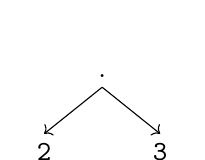
\begin{tikzpicture}
			\tikzset{edge from parent/.append style={->}}
			\tikzset{sibling distance=30pt}
			\Tree [.{.} \edge node[auto=right]{\scriptsize\car}; \Verb+2+ \edge node[auto=left]{\scriptsize{\cdr}}; \Verb+3+ ]
	\end{tikzpicture}
	$$
	\end{uenumi}

\item You can construct a cons of two objects by applying the procedure \Verb+CONS+; for instance, 

\begin{lispcode}
(cons 2 3)
\end{lispcode}

will return a cons of 2 and 3. Witness that 

\begin{lispcode}
(let ((k (cons 2 3)))
    (consp k))
\end{lispcode}

will return \Verb+T+.

You can reach the components of a cons by the built-ins \Verb+CAR+ and \Verb+CDR+:\footnote{Note that instead of giving full top-level interaction, we designate the return value by \Verb+==>+, which is not part of \Verb+LISP+.}

\begin{lispcode}
(let ((k (cons 2 3))) (car k)) ==> 2 
(let ((k (cons 2 3))) (cdr k)) ==> 2 
\end{lispcode}

\end{uenum}

\subsection{Lists}

\begin{uenum}
\item List is the central data structure in LISP, which stands for Lis(t) P(rocessor).
	\begin{uenumi}
	\item Lists are represented as sequences of objects separated by white space and enclosed in parentheses: 
\begin{lispcode}
(1 3 9)
(RED GREEN BLUE)
(1 GREEN)
()
(7)
\end{lispcode}
\end{uenumi}

\item We call an object in a list its element.

\item The empty list is represented in two equivalent ways: \Verb+NIL+ and \Verb+()+ -- both evaluate to themselves.

\item Lists are represented internally as conses. The \car\ of the cons points to the first element of the list, while the \cdr\ of the cons points to the rest of the list (= the list without its first element).

 	\begin{uenumi}
 	\item The single element list \Verb+(7)+ is represented as:
 	
 	$$
 	\begin{tikzpicture}
 		\tikzset{edge from parent/.append style={->}}
 		\tikzset{sibling distance=30pt}
 		\Tree [.{.} \edge node[auto=right]{\scriptsize\car}; \Verb+7+ \edge node[auto=left]{\scriptsize{\cdr}}; \nil{} ]
 	\end{tikzpicture}
 	$$

	\item The two element list \Verb+(2 TWO)+ is represented as:   		
	$$
	\begin{tikzpicture}
		\tikzset{edge from parent/.append style={->}}
		\tikzset{sibling distance=30pt}
		\Tree [.{.} \edge node[auto=right]{\scriptsize\car}; \Verb+2+ \edge node[auto=left]{\scriptsize{\cdr}}; [.{.} \edge node[auto=right]{\scriptsize\car}; \Verb+TWO+ \edge node[auto=left]{\scriptsize{\cdr}}; \nil{} ] ]
	\end{tikzpicture}
	$$
	\item[] and so on\ldots
	\item The only exception to cons-based representation of lists is the empty list, which is the object \Verb+NIL+, which is not a cons. 
	\item Lists can be nested (= lists as elements of lists). 
	\begin{uenumii}
	\item Take for example \Verb+((RED 122) (GREEN 231) (BLUE 15))+:\footnote{From here on we adopt the convention that the left branch leaving a cons is \car\ and the right branch is \cdr, to be able to omit the labels on the edges.}
	$$	
	\begin{tikzpicture}
	\tiny
		\tikzset{edge from parent/.append style={->}}
		\tikzset{level distance=25pt}
		\tikzset{sibling distance=10pt}
		\Tree [.{.} [.{.} \Verb+RED+ [.{.} \Verb+122+ \nil{} ] ] [.{.} [.{.} \Verb+GREEN+ [.{.} \Verb+231+ \nil{} ] ] [.{.} [.{.} \Verb+BLUE+ [.{.} \Verb+15+ \nil{} ] ] \nil{} ]  ] ] 
	\end{tikzpicture}
	$$
	\end{uenumii}
 	\end{uenumi}

\item {\bf \Verb+QUOTE+:} Notice that trying to get the first element of the list \Verb+(1 2 3)+ by \Verb+(car (1 2 3))+ results in error. The reason is that \Verb+SBCL+ attempts to interpret the form \Verb+(1 2 3)+ as an application, seeking a procedure definition under the name \Verb+1+. This is so because \Verb+CAR+ is an application, its argument needs to get evaluated. But in this case we mean a list to be just a list and would not want \Verb+LISP+ to evaluate that expression as a procedure call. To tell \Verb+LISP+ \emph{not} to evaluate an expression and leave it as it is,  put the expression in quotes; just like one does in natural language. The following would behave well:

\begin{lispcode}
(car (quote (1 2 3)))
(cdr (quote (a b c)))
\end{lispcode}

\begin{uenumi}
\item As one needs so frequently to quote expressions, there is a shorthand for \Verb+QUOTE+:

\begin{lispcode}
(car '(1 2 3))
(cdr '(a b c))
\end{lispcode}

\end{uenumi}

\item {\bf Quoting symbols:} Preventing evaluation by quoting applies to symbols as well. This enables one to use symbols as data; a quoted symbol evaluates to the symbol itself.

Note that \Verb+'(a b c)+ is not the same as \Verb+('a 'b 'c)+, make sure that you understand why.

\item {\bf Constructing lists:} The most basic constructor for lists is \Verb+CONS+, it adds an object (\Verb+CAR+) to the front of a list (\Verb+CDR+). Another constructor is \Verb+LIST+, it simply evaluates and collects its operands into a list. Yet another is \Verb+APPEND+, which joins together lists. \Verb+CONS+ is always two argument, while \Verb+LIST+ and \Verb+APPEND+ take as many arguments as they like, including zero. Try and observe the difference between the following:

\begin{lispcode}
(cons '(1 2) '(3))
(list '(1 2) '(3))
(append '(1 2) '(3))
\end{lispcode}

\item {\bf Dotted lists:} In a normal list, as you break down the list into its conses, you will always find a ``bottom'' cons where an object is consed with the empty list \Verb+NIL+. In a dotted list this ``bottom'' cons does not involve \Verb+NIL+. For instance you can cons two non-\Verb+NIL+ objects and form a dotted list:

\begin{lispcode}
(cons 'a 'b) ==> (A . B)
\end{lispcode}

You can go on consing to this dotted list:
\begin{lispcode}
(cons 'x (cons 'a 'b)) ==> (X A . B)
\end{lispcode}

\Verb+SBCL+ will visually indicate a dotted list by a dot before the \Verb+CDR+. Normal lists and dotted lists differ in their final \Verb+CDR+s.

\item {\bf Accessing list elements:} We already know how to access the first element, namely by \Verb+CAR+. What about other elements? One way is to combine \Verb+CAR+s and \Verb+CDR+s. For instance having,

\begin{lispcode}
(defvar k '(1 (2 3) 4))
\end{lispcode}

to get the list \Verb+(2 3)+ you can make \Verb+(car (cdr k))+;\\ or to get 2 \Verb+(car (car (cdr k)))+; or to get 3 \Verb+(car (cdr (car (cdr k))))+.

\Verb+LISP+ provides the built-ins \Verb+FIRST+ to \Verb+TENTH+. Some people like to use \Verb+FIRST+ for \Verb+CAR+ and \Verb+REST+ for \Verb+CDR+.

You can combine the successive \Verb+CAR+s and \Verb+CDR+s as in \Verb+CDDR+ or \Verb+CADAR+ up to a certain level. The convention is to match the nested operators from right to left and inside to outside. For instance \Verb+(cadr x)+ is equivalent to \Verb+(car (cdr x))+, which is equivalent to \Verb+(second x)+.

Finally, the built-in \Verb+NTH+ takes a non-negative integer and a list, and gives the element at that index position, where indexing starts with 0 -- an index out of the range of the list returns \Verb+NIL+. 

\end{uenum}


\noindent\hrulefill

\begin{uexercise}

Construct the lists formed by the below expressions, using only \Verb+CONS+, elements, and \Verb+NIL+ -- do not forget the quotes where needed.

\item \Verb+(list 'a 'b 'c)+ 
\item \Verb+(list 'a 'b NIL)+ 

\qed
\end{uexercise}

\begin{uexercise}

Construct the lists below by using only \Verb+CONS+, elements, and \Verb+NIL+ -- do not forget the quotes where needed.

\item \Verb+(a b x d)+

\item \Verb+(a (b (x d)))+

\item \Verb+(a (b (d) x))+

\item \Verb+(((a (b (x) d))))+

\qed
\end{uexercise}

\begin{uexercise}

Give the sequences of car's and cdr's needed to get \Verb+x+ in the following expressions; for convenience name the list under discussion as \Verb+lst+ -- the first one is answered to clarify the question:
\begin{itemize}
\item \Verb+(a x b d)+

 \Verb+(car (cdr lst))+

\item \Verb+(a b x d)+

\item \Verb+(a (b (x d)))+

\item \Verb+(a (b (d) x))+

\item \Verb+(((a (b (x) d))))+

\end{itemize}

\qed
\end{uexercise}

\begin{uexercise}
Given the list \Verb+((A B) (C D) (E F))+,\footnote{Touretzky, ex. 2.15.} 

\begin{enumerate}
\item Write what you would get from it by applying the following in order,\footnote{Do not directly check on the computer, first attempt it on paper.}
	\begin{enumerate}
	\item \Verb+CAR+
	\item \Verb+CDR CDR+
	\item \Verb+CAR CDR +
	\item \Verb+CDR CAR +
	\item \Verb+CDR CDR CAR +
	\item \Verb+CDR CAR CDR CDR +
	\end{enumerate}

\item Which sequences of \Verb+CAR+s and \Verb+CDR+s would get you \Verb+A+, \Verb+B+ and \Verb+F+?
\end{enumerate}

\qed
\end{uexercise}

\begin{uexercise}

Write down what the following expressions evaluate to; work them out before trying on the computer. Some expressions might cause an error; just mark them as an error, no need to specify the error itself.

\begin{enumerate}
\item \Verb=(cons 2)=
\item \Verb=(cons 2 NIL)=
\item \Verb=(cons 3 '(2))=
\item \Verb=(cons 3 (2))=
\item \Verb=(cons NIL NIL)=
\item \Verb=(cons (1 2) NIL)=
\item \Verb=(cons '(1 2) NIL)=
\item \Verb=(cons (A B) NIL)=
\item \Verb=(cons ('A 'B) NIL)=
\item \Verb=(cons '(A B) NIL)=
\item \Verb=(cons '(A B) '(C D))=
\item \Verb=(list 1 4)=
\item \Verb=(list 1 '4)=
\item \Verb=(list '1 4)=
\item \Verb=(list 'A B)=
\item \Verb=(list 'A 4)=
\item \Verb=(list 'A 'B)=
\item \Verb=('list 1 4)=
\item \Verb=(+ 3 '4)=
\item \Verb=('+ 1 4)=
\item \Verb=(list 3 'times '(- 5 2) 'is 9)=
\item \Verb=(list 3 'times (- 5 2) 'is '9)=
\end{enumerate}

\qed
\end{uexercise}

\begin{uexercise}
Write down what the following expressions evaluate to; work them out before trying on the computer.

\begin{enumerate}
\item \Verb=(if (listp '(list 1 2)) 'ok 'not-really)=
\item \Verb+(if (null (nil)) 'vice 'versa)+
\item \Verb=(and (listp (if (> 2 4) (- 2 4) (+ 2 4)))=\\
\Verb=(if (> 2 4) (- 2 4) (+ 2 4)))=
\item \Verb=(or (listp (if (> 2 4) (- 2 4) (+ 2 4)))=\\
\Verb=(if (> 2 4) (- 2 4) (+ 2 4)))=
\item \Verb=(or (and (or 'or) 'and) 'or)= 
\end{enumerate}

\qed
\end{uexercise}

\begin{uexercise}[*]

The Collatz sequence (see Exercise~\ref{collatzdef}) of a positive integer is the sequence
starting with the number itself and ending with 1, where the numbers
in-between are the results of Collatz steps. For instance the Collatz
sequence of 3 is 3 10 5 16 8 4 2 1.

Given a non-negative integer, compute the count of even and odd
numbers in its Collatz sequence. Return the result as a
list of two numbers, the first  is the even count and the
second is the odd count. The solution for 3 will be (5 3).
\qed
\end{uexercise}


\noindent\hrulefill

\subsection{Procedures on lists}

\begin{uenum}

\item {\bf Example (membership):} \Verb+LISP+ has a built-in membership procedure called \Verb+MEMBER+ for lists. Let's define our own:

\begin{lispcode}
(defun memberp (item lst)
  (cond ((endp lst) nil) ; test if lst is empty or not
        ((equal item (car lst)) t)
        (t (memberp item (cdr lst)))))
\end{lispcode}

\item {\bf List predicates:}
\begin{uenumi}
\item {\bf \Verb+NULL+ vs. \Verb+ENDP+:}
Note that the test for emptiness of a list is \Verb+ENDP+. There is another predicate \Verb+NULL+ which behaves quite like \Verb+ENDP+, giving \Verb+T+ for \Verb+NIL+. The two predicates diverge in their behavior for non \Verb+NIL+ inputs. \Verb+NULL+ gives \Verb+NIL+ for anything that is not \Verb+NIL+; but \Verb+ENDP+ gives an error if its argument is not a list. 

\item {\bf \Verb+LISTP+ vs. \Verb+CONSP+:} Any cons will answer \Verb+T+ to \Verb+CONSP+. All lists are conses with the only exception of \Verb+NIL+. Therefore, \Verb+NIL+  is the only thing that will answer \Verb+NIL+ to \Verb+CONSP+ and \Verb+T+ to \Verb+LISTP+. Yes, a little complicated; make sure you get it right.

There is also \Verb+ATOM+, which is a predicate\footnote{Note that \Verb+NULL+ and \Verb+ATOM+ do not follow the general convention of ending predicate names with `p'.} that answers \Verb+T+ to expressions that answer \Verb+NIL+ to \Verb+CONSP+. 
\end{uenumi}

\item {\bf Example (length):} Now our own version of the built-in \Verb+LENGTH+, first without an accumulator:

\begin{lispcode}
(defun len (lst)
  (if (endp lst)
    0
    (+ 1 (len (cdr lst)))))
\end{lispcode}

and now with an accumulator:

\begin{lispcode}
(defun len-acc (lst &optional (counter 0))
  (if (endp lst)
    counter
    (len-acc (cdr lst) (+ counter 1))))
\end{lispcode}


\end{uenum}


\noindent\hrulefill

\begin{uexercise}
Define a procedure named \Verb+INSERT-2ND+, which takes a list and an object, and gives back a list where the element is inserted after the first element of the given list. Assume that the input list will have at least one element. Here is a sample interaction:

\begin{lispcode}
* (insert-2nd 'b '(a c))

(A B C)
* (insert-2nd '(b k) '(a c))

(A (B K) C)
* 
\end{lispcode}

\qed
\end{uexercise}

\begin{uexercise}

Define a procedure \Verb+SWAP+, that takes a two element list and switches the order of the elements. You are allowed to use only \Verb+CAR+, \Verb+CDR+, \Verb+CONS+ and \Verb+NIL+ as built-ins.
\qed
\end{uexercise}

\begin{uexercise}
Define a procedure that takes a list and an object, and returns a list where the object is added to the end of the list.

\qed
\end{uexercise}

\begin{uexercise}
Define your own procedure \Verb+APPEND2+ that appends two list arguments into a third list. You are not allowed to use \Verb+APPEND+, \Verb+LIST+ and \Verb+REVERSE+ -- use just \Verb+CONS+.

\qed
\end{uexercise}

\begin{uexercise}
Using \Verb+CAR+ and \Verb+CDR+, define a procedure to return the fourth element of a list.\footnote{Graham (1996), p.\ 29, ex.\ 3.} 

\qed
\end{uexercise}

\begin{uexercise}
Define a procedure named \Verb+REPLACE-2ND+, which is like \Verb+INSERT-2ND+, but \emph{replaces} the element at the 2nd position. Assume that the input list will always have at least two elements.

\qed
\end{uexercise}

\begin{uexercise}
Define a procedure \Verb+AFTER-FIRST+ that takes two lists and inserts all the elements in the second list after the first element of the first list. Given \Verb+(A D E)+ and \Verb+(B C)+, it should return \Verb+(A B C D E)+.
\qed
\end{uexercise}

\begin{uexercise}
The procedure \Verb+WRAP-2+ takes a two element list, and wraps each element inside a list: 

\begin{lispcode}
* (wrap-2 '(a (b)))

((A) ((B)))
* (wrap-2 '(a b))

((A) (B))
* (wrap-2 (wrap-2 '(a b)))

(((A)) ((B)))
* (wrap-2 (wrap-2 (wrap-2 '(a b))))

((((A))) (((B))))
* 
\end{lispcode}

Write two versions of \Verb+WRAP-2+:

\begin{enumerate}
\item one using \Verb+LIST+, \Verb+CAR+ and \Verb+CADR+
\item the other using \Verb+CONS+, \Verb+CAR+ and \Verb+CADR+
\end{enumerate}

\qed
\end{uexercise}


% \begin{uexercise}
% The built-in \Verb+MEMBER+ takes and object and a list and checks whether the  object appears in the list or not; discover how it works. Using \Verb+MEMBER+, define  a function \Verb+MY-MEMBER+ that behaves as follows: 
% 
% {\small
% \begin{Verbatim}
% * (my-member 'b '(a b c))
% 
% (B IS A MEMBER OF (A B C))
% * (my-member 'z '(a b c))
% 
% (Z IS NOT A MEMBER OF (A B C))
% * 
% \end{Verbatim}
% }
% 
% \qed
% \end{uexercise}

\begin{uexercise}
Assume you have data that pairs employees' last names with their
monthly salaries. E.g.\ \Verb+((SMITH 3000) (JOHNS 2700) (CURRY 4200))+ Define a procedure that takes as input employee data and a threshold salary (an integer), and returns in a list the last names of all the employees that earn above the threshold salary. Define two versions, one with, and one without an accumulator.

\qed
\end{uexercise}

\begin{uexercise}
\label{order}
Using \Verb+MEMBER+  and \Verb+LENGTH+, write a function \Verb+ORDER+ which gives the order of an item in a list. You can do this by combining \Verb+LENGTH+ and \Verb+MEMBER+ in a certain way. It should behave as follows:

{\small
\begin{Verbatim}
* (order 'a '(a b c))

1
* (order 'c '(a b c))

3
* (order 'z '(a b c))

NIL
\end{Verbatim}
}

\qed
\end{uexercise}

\begin{uexercise}
Define a procedure that computes the sum of a list of numbers; with
and without an accumulator. Consider that there might be non-number
elements in a list, which you should ignore in your summation.

\qed
\end{uexercise}

\begin{uexercise}
Define a procedure that returns the largest number in a list of numbers. Do not use the built-in \Verb+MAX+.

\qed
\end{uexercise}

\begin{uexercise}
Define a procedure that takes a list of integers and returns the \emph{second} largest integer in the list.

\qed
\end{uexercise}

\begin{uexercise}
Define a procedure that takes a list of integers and an integer $n$, and returns the $n$th largest integer in the list.

\qed
\end{uexercise}

\begin{uexercise}
\label{exlast}
Define a procedure that gives the last element of a list or gives NIL if the list is empty. Name your procedure  \Verb+LASTT+ in order not to clash with  \Verb+LISP+'s built-in \Verb+LAST+. 

\qed
\end{uexercise}

\begin{uexercise}
Define a procedure \Verb+MULTI-MEMBER+ that checks if its first argument occurs more than once in the second.

\qed
\end{uexercise}

\begin{uexercise}

Define a recursive member procedure that checks whether a given item is found in the given list. The item is not required to be a top-most element. Some sample interactions are as follows:

\begin{Verbatim}
* (rec-mem 'a '(b a c))
t
* (rec-mem 'a '(b (z a k) c))
t
* (rec-mem 'a '(b (z (a x) k) c))
t
\end{Verbatim}

\qed
\end{uexercise}

\begin{uexercise}[*]

Define a procedure \Verb+LEVEL+, that takes an element \Verb+X+ and a
list \Verb+LST+, and returns the level of depth that \Verb+X+ is found
in \Verb+LST+. If \Verb+X+ is not a member, your procedure will return
\Verb+NIL+. Top level counts as 0, every level of nesting adds 1 to
the depth. Sample interaction:

\begin{Verbatim}
* (level 'a '(b a c))
0
* (level 'a '(b (z a k) c))
1
* (level 'a '(b (z (a x) k) c))
2
\end{Verbatim}

\qed
\end{uexercise}

\begin{uexercise}[*]

Given a possibly nested list of symbols one and only one of which will
be the symbol \Verb+X+, compute the steps of \Verb+CAR+s and
\Verb+CDR+s required to get \Verb+X+ from the list.  For instance, the
input \Verb+((a (z x d)) (c s d))+ must yield the result \Verb+(CAR CDR CAR CDR CAR)+.  

\qed
\end{uexercise}

\begin{uexercise}
Define a procedure \Verb+NESTEDP+ that takes a list and returns \Verb+T+ if at least one of its elements is a list, and returns \Verb+NIL+ otherwise.\footnote{Graham 1996, p.\ 30 ex.\ 7.}

\qed
\end{uexercise}

\begin{uexercise}

Define a recursive function \Verb+FLATTEN+, which takes a possibly nested list and returns a version where all nesting is eliminated. E.g.\ \Verb+((1 (2) 3) 4 (((5) 6) 7))+ should be returned as \Verb+(1 2 3 4 5 6 7)+. 

\qed
\end{uexercise}

\begin{uexercise}
Define a procedure \Verb+SPLIT+ that takes an integer $n$ and a list, and returns a list of two lists such that the first has the first $n$ elements of the input list, and the second has the rest of the elements of the input list. Do NOT use \Verb+LENGTH+.

\qed
\end{uexercise}

\begin{uexercise}
Define a procedure \Verb+SPLIT-TWO+ that splits a list of numbers into two equal length lists. If the original list has an odd length, there will be a middle element. Split this middle element between the two halves; half of it goes to the end of the first list, half of it goes to the beginning of the second list.

\qed
\end{uexercise}

\begin{uexercise}
\label{halve}

Define a procedure \Verb+HALVE+ that splits a list into two. If the
length is odd, let one of the halves be one item longer than the
other. (You can use length, if you like.)  For instance, \Verb+(split '(a b c d e f g h i j k l))+
must give \Verb+((A B C D E F) (G H I J K L))+.

\qed
\end{uexercise}

\begin{uexercise}[*]
Write a program named \Verb+RANGE+, that takes a non-negative integer
\Verb+N+ as argument and returns a list of non-negative integers that
are less than \Verb+N+ in increasing order.  Here is a sample
interaction with the first four non-negative integers, your solution
must work for all non-negative integers: 

\begin{lispcode}
CL-USER> (range 0)
NIL
CL-USER> (range 1)
(0)
CL-USER> (range 2)
(0 1)
CL-USER> (range 3)
(0 1 2)
\end{lispcode}

\begin{itemize}
\item[a.] Solve the problem without using an accumulator;
\item[b.] Solve the problem using an accumulator.
\end{itemize}

\qed
\end{uexercise}

\begin{uexercise}[*]
Write a program that takes a sequence, a start index, an end index
and returns the sub-sequence from start to (and including) end.
Indices start from 0.

\qed
\end{uexercise}

\begin{uexercise}[*]
Write a program that takes two parameters \Verb+count+ and \Verb+max+,
and returns a list of \Verb+count+ random integers, all less than
\Verb+max+.

\qed
\end{uexercise}

\begin{uexercise}
\label{reverse}
The built-in \Verb+REVERSE+ reverses a list. Define your own version of reverse.
\qed
\end{uexercise}

\begin{uexercise}

In Ex \ref{reverse} you defined a list reversing procedure. Now alter that definition so that it  not only reverses the order of the top-level elements in the list but also reverses any members which are themselves lists.

{\small
\begin{Verbatim}
* (reverse0 '(a (b c (x d)) k))
(K ((D X) C B) A)
\end{Verbatim}
}
\qed
\end{uexercise}

% \begin{uexercise}
% Define a predicate that tells whether its argument is a dotted list or not.
% \qed
% \end{uexercise}

\begin{uexercise}

Define a procedure \Verb+HOW-MANY?+ that counts the top-level occurrences of an item in a list.

\begin{Verbatim}
(how-many? 'a '(a b r a c a d a b r a))
5
\end{Verbatim}
\qed
\end{uexercise}

\begin{uexercise}
Define a recursive procedure \Verb+D-HOW-MANY?+ that counts all – not only top-level – occurrences of an item in a list.\\ For instance \Verb+(D-HOW-MANY? 'A '((A B) (C (A X)) A))+ should return 3. 
\qed
\end{uexercise}


\begin{uexercise}
Define a three argument procedure \Verb+REMOVE-NTH+, which removes every $n$th occurrence of an item from a list.
\qed
\end{uexercise}


\begin{uexercise}
A given set $A$ is a {\bf subset} of another set $B$ if and only if all the members of $A$ are also a member of $B$. Two sets are {\bf equivalent}, if and only if they are subsets of each other. For this problem you will represent sets via lists.

\begin{enumerate}
\item Define a procedure \Verb+SUBSETP+ that takes two list arguments and decides whether the first is a subset of the second.
\item Define a procedure \Verb+EQUIP+ that takes two list arguments and decides whether the two are equivalent.
\item Define a procedure \Verb+IDENP+ that takes two list arguments and decides whether the two have the same elements in the same order -- do not directly compare the lists with \Verb+EQUALP+, you are required to do a element by element comparison.
\end{enumerate}

\qed
\end{uexercise}

\begin{uexercise}
Define a procedure \Verb+REMOVE2+ that takes an element and a list; and returns a list where all the occurrences of the element are removed from the list.

\qed
\end{uexercise}

\begin{uexercise}[*]
 Given a sequence of 0s and 1s, return the number of 0s that
are preceded by a 0. Here is a sample interaction:

\begin{lispcode}
CL-USER> (zeros '(0))
0
CL-USER> (zeros '(0 0))
1
CL-USER> (zeros '(1 0 1))
0
CL-USER> (zeros '(1 0 0 0 1 0))
2
\end{lispcode}

\qed
\end{uexercise}

\begin{uexercise}
Define a procedure \Verb+REMAFTER+  that takes an element, a list and
a pivot element; and returns a list where all the occurrences of the
element that are preceded by the pivot element are removed from the list.

\qed
\end{uexercise}

% \begin{uexercise}
% Define a procedure \Verb+TYPES+ that takes a list and prints out the type of the elements encountered. It's enough that it can tell between number, list and symbol; so use \Verb+NUMBERP+, \Verb+LISTP+ and \Verb+SYMBOLP+. In case you cannot match to any of these, print \Verb+UNKNOWN-TYPE+.  Put a string in your list for testing, it answers \Verb+NIL+ to all these predicates.
% 
% \qed
% \end{uexercise}

\begin{uexercise}
The mean of $n$ numbers is computed by dividing their sum by $n$. A running mean is a mean that gets updated as we encounter more numbers. Observe the following input-output sequences:

\begin{Verbatim}
* (run-mean '(3 5 7 9))
(3 4 5 6)
\end{Verbatim}

The first element 3 is the mean of the list \Verb+(3)+, the second element 4 is the mean of \Verb+(3 5)+, and so on. Implement \Verb+RUN-MEAN+ by using \Verb+DOTIMES+ and \Verb+NTH+.

\qed
\end{uexercise}

\begin{uexercise}
		\label{chaindef}

A chain in a sequence of numbers is such that each number in the chain is either equal to or greater than the one before it. For instance, 2 5 9 12 17 21 is a chain, but not 2 5 9 17 12 21, because the 17 12 sub-sequence breaks the chain. Define a recursive procedure that finds and returns the longest chain in a sequence of numbers. If there are more than one sequences with the highest length, return the one you encountered first. Here are some sample interactions:

\begin{Verbatim}
* (longest-chain '(14 3 8 27 25 12 19 3 1))
(3 8 27)
* (longest-chain '(14 3 8 27 25 12 19 34 42 1))
(12 19 34 42)
* (longest-chain '(14 3 8 27 25 12 19 34 1))
(3 8 27)
\end{Verbatim}

\qed
\end{uexercise}

\begin{uexercise}[*]

A maximal chain $m$ in a sequence of integers $I$ is a chain defined
in the sense of Exercise~\ref{chaindef}, such that there is no chain
$k$ in $I$ such that $m$ is a subsequence of $k$. 

Define a procedure which takes a sequence of integers and returns the
maximal chain with the largest sum. If you detect maximal chains with
equal sums, return the one you encountered first.

\qed
\end{uexercise}

\begin{uexercise}[*]

Define a procedure which takes a sequence of integers and returns the
chain  -- not necessarily maximal -- with the largest sum. If you
detect maximal chains with equal sums, return the one you encountered
first.

\qed
\end{uexercise}

\begin{uexercise}
See the \Verb+PAIRLISTS+ in lecture notes. Define a procedure that ``pairs'' an arbitrary number of lists. Here is a sample interaction:

{\small
\begin{Verbatim}
* (pairlists '((a b) (= =) (1 2) (+ -) (3 9)))
((A = 1 + 3) (B = 2 - 9))
\end{Verbatim}
}

\qed
\end{uexercise}

\begin{uexercise}
Define a procedure \Verb+SEARCH-POS+ that takes a list as search item, another list as a search list and returns the list of positions that the search item is found in the search list. Positioning starts with 0. A sample interaction:

{\small
\begin{Verbatim}
* (search-pos '(a b) '(a b c d a b a b))
(6 4 0)
* (search-pos '(a a) '(a a a a b a b))
(2 1 0)
\end{Verbatim}
}

\qed
\end{uexercise}

\begin{uexercise}
Define a procedure \Verb+LAST2+ that takes a list and returns the last element of the list. Of course, don't use \Verb+LAST+. One way could be to keep a counter, so that you can compare this to the length of the list to recognize whether you are close enough to the end of the list.

\qed
\end{uexercise}

\begin{uexercise}
Define an iterative procedure \Verb+CHOP-LAST+, which removes the final element of the given list -- its like \Verb+CDR+ from the back. You are NOT allowed to make\\ \Verb+(REVERSE (CDR (REVERSE LST)))+. Nothing to be done for an empty list, just return it as it is; but a single element list gets ``nilled''.

\qed
\end{uexercise}

\begin{uexercise}
Define a procedure that checks whether a given list of symbols is a palindrome. Use \Verb+CAR+ and your solution to Ex.\ \ref{exlast}.
\qed
\end{uexercise}

\begin{uexercise}
Define your own version of \Verb+NTH+ (don't use \Verb+NTHCDR+).
\qed
\end{uexercise}


\begin{uexercise}
\label{uniq}
Define a procedure \Verb+UNIQ+ that takes a list and removes all the repeated elements in the list keeping only the first occurrence. For instance:

\begin{Verbatim}
* (uniq '(a b r a c a d a b r a))
(A B R C D)
\end{Verbatim}

Don't use \Verb+REMOVE+ (built-in or in-house), you may use \Verb+MEMBER+.
\qed
\end{uexercise}

\begin{uexercise}
Solve Ex \ref{uniq} by keeping the last occurrence rather than the first.
\qed
\end{uexercise}

\begin{uexercise}
Define a procedure \Verb+REMLAST+ which removes the last occurrence of an item from a list. Do not use \Verb+MEMBER+ or \Verb+REVERSE+.
\qed
\end{uexercise}

\begin{uexercise}

Define a procedure \Verb+REMOVEX+  that takes an element and a list; and returns a list where all the occurrences of the element that are preceded by the symbol \Verb+X+ are removed from the list.
\qed
\end{uexercise}

\begin{uexercise}
Define a function \Verb+ROTATE-LEFT+ that takes a list and moves the first element to the end of the list. For instance, \Verb+(ROTATE-LEFT '(1 2 3))+ should give \Verb+(2 3 1)+, \Verb+(ROTATE-LEFT '(1 2))+ should give \Verb+(2 1)+, etc. Apart from \Verb+DEFUN+, you are allowed to use \Verb+LET+, \Verb+LIST+, \Verb+APPEND+, \Verb+CAR+, \Verb+DOLIST+, \Verb+SETF+ and \Verb+IF+. No other function is available for use.

\qed
\end{uexercise}


\begin{uexercise}

Define a recursive  procedure \Verb+SUBSTITUTE+, with 3 arguments, say \Verb+old+ \Verb+new+ \Verb+exp+ such that every occurrence of \Verb+old+ at the top-level of \Verb+exp+ is replaced by \Verb+new+. By ``top-level'' we mean the function should not check embedded levels in lists. E.g.\ \Verb+(substitute 'x 'k '(x (x y) z))+ should return \Verb+(k (x y) z)+.

\qed
\end{uexercise}

\begin{uexercise}

Define a procedure \Verb+MATCHES+ that takes two lists, a pattern and a text, and returns the count of the occurrences of the pattern in the text. You need to be careful about overlapping matches. For instance, \Verb+(A C A)+ has 3 occurrences in \Verb+(A C A C A T G C A C A T G C)+. You are not allowed to use procedures like \Verb+SUBSEQ+ to take portions of the text for comparison; your solution must go through the text element by element.

\qed
\end{uexercise}

\begin{uexercise}
Define a procedure \Verb+SHUFFLE+ that takes a list and returns a random permutation of the list. A random permutation of a list is one of all the possible orderings of the elements of the list. You can follow any strategy you like -- recursive or iterative.
You might find two built-ins especially useful: \Verb+RANDOM+ takes an integer and gives a random number from 0 to one less than the given integer; \Verb+NTH+ takes an integer and a list, returning the element at the position of the given integer -- remember that positions are counted starting from 0.

\qed
\end{uexercise}

\begin{uexercise}

Modify \Verb+SUBSTITUTE+ to \Verb+D-SUBS+ (for ``deep substitute''), so that it does the replacement for \emph{all} occurrences of \Verb+old+, no matter how deeply embedded.
\qed
\end{uexercise}

\begin{uexercise}

Define a recursive procedure that counts the non-nil atoms  in a list. For instance, an input like \Verb+((a b) c)+ should return 3, \Verb+(a ((b (c) d)))+ should return 4, and so on. Remember that the  built-in \Verb+ATOM+ returns \Verb+NIL+ for all lists except \Verb+NIL+; \Verb+NULL+ returns \Verb+T+ only for \Verb+NIL+; \Verb+ENDP+ is like \Verb+NULL+, except that it gives an error if its input happens to be something other than a list. Your function should use a counter/accumulator -- it will be a two argument function.
\qed
\end{uexercise}

\begin{uexercise}
Define a procedure \Verb+BRING-TO-FRONT+ (or \Verb+BFT+ for short), that takes an item and a list and returns a version where all the occurrences of the item in the given list are brought to the front of the list.\\ For instance, 
\Verb+(bring-to-front 'a '(a b r a c a d a b r a))+ would return\\ \Verb+(A A A A A B R C D B R)+;\\ and \Verb+(bring-to-front 'b '(a b r a c a d a b r a))+ would return \\ \Verb+(B B A R A C A D A R A)+.\\ You are NOT allowed to count the occurrences of the item in the given list or use \Verb+REMOVE+.
\qed
\end{uexercise}

\begin{uexercise}
Define a procedure that groups the elements in a list putting consecutive occurrences of items in lists. For instance, \Verb+(group '(a a b c c c d d e))+ should give \Verb+((A A) (B) (C C C) (D D) (E))+. Note that you should NOT bring together non-consecutive repetitions; a call like  \Verb+(group '(a b b c b b c))+ should return \Verb+((A) (B B) (C) (B B) (C))+.
\qed
\end{uexercise}


\begin{uexercise}
Define a version of Exercise~\ref{halve} without using \Verb+LENGTH+ -- here we go again!

\qed
\end{uexercise}

\begin{uexercise}[*]
Define a recursive procedure \Verb+SUMMARIZE+, that takes a list and returns a list of pairs whose car is an element in the list and cadr is the number of times the element occurs in the list; \Verb+(summarize '(a b r a c a d a b r a))+ should give \Verb+((a 5) (b 2) (r 2) (c 1) (d 1))+.

\qed
\end{uexercise}

\begin{uexercise}

A growing difference sequence is a recursive sequence where each non-initial term in the sequence is greater than the one before it by a difference that steadily grows with the terms. For instance 1, 4, 8, 13, 26,\ldots is such a sequence where the second term is obtained by adding 3 to the first, third term is obtained by adding 4 to the second, fourth term is obtained by adding 5 to the third, and so on. In tabular form:

\begin{tabular}{|c|c|c|}
\hline 
index & term & difference \\
\hline
1 & 1 & 3 \\
\hline
2 & 4 & 4 \\
\hline
3 & 8 & 5 \\ 
\hline
4 & 13 & 6 \\
\hline
5 & 19 & 7 \\
\hline
6 & 26 & 8 \\
\hline
7 & 34 & 9 \\
\hline
$\vdots$ & $\vdots$ & $\vdots$
\end{tabular}

Our sequences will always start with 1. How the difference starts and grows may change from sequence to sequence. For instance the difference in the following sequence starts with 2 and grows as the square of the previous difference.

\begin{tabular}{|c|c|c|}
\hline 
index & term & difference \\
\hline
1 & 1 & 2 \\
\hline
2 & 3 & 4 \\
\hline
3 & 7 & 16 \\ 
\hline
4 & 23 & 256 \\
\hline
5 & 279 & 65536 \\
\hline
$\vdots$ & $\vdots$ & $\vdots$
\end{tabular}

Define a procedure \Verb+GDS+ that generates a growing difference sequence where the length of the sequence, the initial value of the difference and how difference grows will be given as parameters. An example output for the first 7 terms in the first example above would be \Verb+((1 1) (2 4) (3 8) (4 13) (5 19) (6 26) (7 34))+.

\qed
\end{uexercise}

\begin{uexercise}
As you have observed, the recursive solution to the computation of $n$th Fibonacci number is quite inefficient, as you compute the same Fibonacci numbers multiple times. Such algorithms can be made efficient by using a technique called \emph{memoization}. The basic idea in memoization is to store the result of some computations in a table, so that when the function is called with some arguments already seen, the result is looked up from the table instead of executing the function again.

Your task in this exercise is to make the recursive Fibonacci solution by using memoization. You are required the results computed so far in a \emph{hash table}. Hash tables are dictionaries that keep \emph{key},\emph{value} pairs. In your case the keys will be integers and the value corresponding to a certain key $n$ will be the $nth$ Fibonacci number. In order to learn how hash tables are constructed and managed, please refer to the relevant chapter of one of the books listed on the course website.

You will change your recursive Fibonacci solution in such a way that when called with a certain integer, you will first check whether you have computed this Fibonacci number before by looking at your table, and enter into recursion only in case you do not have the number in the table.

Your procedure will be used exactly as the original one, namely it should be a single argument procedure that takes an integer and return the corresponding Fibonacci number. 

\qed
\end{uexercise}

\begin{uexercise}
Define a procedure \Verb+PERMUTE+ that gives the permutation of a sequence -- all the sequences with the same elements in different orders. Assume all the elements in the sequence will be distinct.

\qed
\end{uexercise}

\begin{uexercise}
Define a procedure that takes a list and turns it into a binary search tree. A binary search tree is a binary tree such that for each node in the tree, all the items in its left sub-tree is less than or equal to the item on that node, and all the items on its right sub-tree are greater than the item on that node. To makes things a little easier you may assume that every node has exactly two sub-trees, which are possibly \Verb+NIL+. You can represent trees in \Verb+LISP+ as lists of three elements; where the first element is the parent node, the second element is the left child and the third element is the right child.

\qed
\end{uexercise}

\begin{uexercise}[*]
Write a program that computes the subsequence with the largest sum in
a sequence of integers.

\qed
\end{uexercise}


\noindent\hrulefill
\newpage

\section{More on symbols}

\begin{uenum}
\item Symbols are more complicated than they first appear to be: 

\renewcommand{\arraystretch}{2.4}
\begin{tabular}{|l|}
\hline
{Name} \\ \hline
{Value Binding} \\ \hline
{Function Binding}\\ \hline 
Package Binding\\ \hline
\end{tabular}

\item To set the Value Binding for a symbol, say \Verb+K+:

\begin{lispcode}
(setf k (random 10)) 
\end{lispcode}

\item Note that \Verb+SETF+ also does not obey the rule of evaluation.

\item \Verb+SETF+ and \Verb+LET+ establish the value binding of a symbol.
\item \Verb+DEFUN+ establishes the function binding of a symbol.
\item A symbol gets evaluated to its value binding, unless it appears as the first element of an unquoted list, in which case it gets evaluated to its function-binding.
\item If you want to access the function binding of a symbol elsewhere, you need to prefix the symbol with \Verb+#'+. More on these rules below.
\item Study the following interaction:

\begin{ucodeframe}
\begin{Verbatim}
* (defvar k 8)
K
* (defun k (x) (* x x))
K
* (symbol-name 'k)
"K"
* (symbol-value 'k)
8
* (symbol-function 'k)
#<FUNCTION K>
* (k k)
64
\end{Verbatim}
\end{ucodeframe}

% \item Second argument of \Verb+SETF+ can make use of the first:
% 
% \begin{lispcode}
% (defvar k)
% (setf k 8)
% (setf k (+ k 3))
% \end{lispcode}
% 
% \item At first glance \Verb+SETF+ might seem to be a simple function which takes a symbol and a value and associates the value-binding of the symbol with the value. Actually it is more clever than that. Observe the following interaction with \Verb+SBCL+:
% 
% \begin{lispcode}
% * (defvar k)
% 
% K
% * (setf k '(A B C))
% 
% (A B C)
% * (setf (car k) 'Z)
% 
% Z
% * k
% 
% (Z B C)
% * 
% \end{lispcode}
% 
% \item \Verb+SETF+ takes two \emph{expressions} and make sure that they evaluate to the same thing.
% \item Also notice that \Verb+SETF+ itself has a return value -- can you see what?
% \item Therefore, \Verb+SETF+ does two things at the same time: manipulates some bindings in the memory and returns a value. The first is called a ``side effect'' of \Verb+SETF+ -- a little bit confusing given the daily usage of the expression.
% \item Knowing the side effects and return values of constructs is crucial.
% \begin{uenumi}
% \item Assume you want to write a function that takes a number and a list, and replaces the first element of the list with the number, in case the number is odd. Here is one way to do it:  
% \begin{lispcode}
% (defun replace-if-odd (a-number a-list)
%   (if (oddp a-number)
% 	(setf (car a-list) a-number)))
% \end{lispcode}
% 
% \item Now also assume that you have some reason to check the length of the list after the replacement. You can check the length of a list by the built-in \Verb+LENGTH+. You do this:
% \begin{lispcode}
% (length (replace-if-odd 3 '(1 2 3)))
% \end{lispcode}
% and you get an error -- can you see why?
% 
% \item Here is a way to make our function return the modified list, so that we can immediately check its length:
% 
% \begin{lispcode}
% (defun replace-if-odd (a-number a-list)
%   (if (oddp a-number)
% 	(cons a-number (cdr a-list))
% 	a-list))
% \end{lispcode}
% 
% \item This time, however, we lost the modified list; we will see a way to both manipulate the list (in-place) and return a value.
% \end{uenumi}

\end{uenum}


\section{Higher order procedures}

\begin{uenum}
\item Assume you have a list of integers that you would want to turn into a list of their, say, factorials in a single stroke. And further assume that you would like to have a more general tool, which does the same trick not only with factorial but any unary function you provide to it, e.g.\ cube, square root, etc. What you need is a function that takes a function and a list as arguments, apply the function one by one to the elements of the list while storing the results in another list. Let us call this function \Verb+MAPP+ -- note the double `P' not to clash with the built-in function \Verb+MAP+.

\begin{uenumi}
\item This is a task that would be straightforwardly implemented with recursion. Assume \Verb+MAPP+ is given a function \Verb+f+ and some list. If the list is empty, than its \Verb+MAPP+ should be empty; if the list is non-empty the \Verb+MAPP+ of it is simply the value obtained by applying \Verb+f+ to the \Verb+CAR+ of the list consed with the value obtained by calling \Verb+MAPP+ with \Verb+f+ and the rest of the list.
\item Here is a definition that attempts to achieve this:

\begin{lispcode}
(defun mapp (func lst) ;; WRONG!
  (if (endp lst)
	nil
	(cons (func (car lst))
	      (mapp func (cdr lst)))))
\end{lispcode}

\item The problem with the above definition is that it expects \Verb+LISP+ to bind the function provided by the parameter \Verb+func+ to the \Verb+func+ that occurs in the function definition. \Verb+LISP+ is designed \emph{not} to do this;\footnote{A dialect of \Verb+LISP+, called \Verb+Scheme+, does this.} when you call this function, say with \Verb+(mapp factorial '(1 2 3 4))+, or \Verb+(mapp 'factorial '(1 2 3 4))+, the \Verb+func+ in the definition will not get replaced by the parameter you provided for the argument named \Verb+func+. Such replacements are done only with non-initial elements of lists -- even not for all such elements, see \ref{stillwrong} below. 

\item What we want is achievable with the functions \Verb+FUNCALL+ or \Verb+APPLY+.

\item\label{funcallspec} \Verb+FUNCALL+ wants its first argument to be something that would \emph{evaluate} to:
\begin{itemize}
\item[i.] a symbol with a function binding; or 
\item[ii.] a function.
\end{itemize}
\item The rest of its arguments are treated as arguments of the function provided via the first argument; the function is applied to its arguments and the value is returned.


\begin{uenumi}

\item Assuming the definition of \Verb+FACTORIAL+ is loaded, 

\begin{ucodeframe}
\begin{Verbatim}
(funcall factorial 8)
\end{Verbatim}
\end{ucodeframe}
would lead to an error. The reason is that before getting fed into \Verb+FUNCALL+ the argument \Verb+FACTORIAL+ gets evaluated. Remember the rule of evaluation, which says that if a symbol is encountered at a non-initial position in a list, it gets evaluated to its value-binding. In this case \Verb+LISP+ cannot find anything in the value-binding. The above specification of \Verb+FUNCALL+ says that the first argument should be something that would \emph{evaluate} to a symbol with a function binding. Therefore the correct form is:

\begin{ucodeframe}
\begin{Verbatim}
(funcall 'factorial 8)
\end{Verbatim}
\end{ucodeframe}

This way \Verb+FUNCALL+ gets a symbol -- that's what \Verb+'FACTORIAL+ gets evaluated to -- with a function-binding. This function is retrieved and applied to the remaining arguments -- we have only one in the present case.

\item You can use the built-in procedures as follows:

\begin{ucodeframe}
\begin{Verbatim}
(funcall '+ 8 7 29)
(funcall 'member 'a '(z c a t))
\end{Verbatim}
\end{ucodeframe}

\item The specification of \Verb+FUNCALL+ in \ref{funcallspec} has a second clause, which says that one can also provide an argument that evaluates to a function. Given a symbol, you can access its function-binding in two ways:

\begin{ucodeframe}
\begin{Verbatim}
(function factorial)
(symbol-function 'factorial)
\end{Verbatim}
\end{ucodeframe}

note the quote in the second form. The first form is the frequent one and like the \Verb+QUOTE+ function, it has an abbreviated form:

\begin{ucodeframe}
\begin{Verbatim}
#'factorial
\end{Verbatim}
\end{ucodeframe}

Therefore you can directly send a function as an argument to \Verb+FUNCALL+ as,

\begin{ucodeframe}
\begin{Verbatim}
* (funcall #'+ 8 7 29)
* (funcall #'factorial 9)
\end{Verbatim}
\end{ucodeframe}

\end{uenumi}


\item\label{stillwrong} Now you might think that with the below code we could get what we want, for instance with

\Verb+(mapp factorial '(1 2 3 4))+

we get \Verb+(1 2 6 24)+. 

{\small
\begin{lispcode}
(defun mapp (func lst) ; STILL WRONG!
  (if (endp lst)
	nil
	(cons (funcall (function func) (car lst))
	      (mapp func (cdr lst)))))
\end{lispcode}
}
but again \Verb+FUNCTION+ -- \Verb+QUOTE+ is no different -- prevents the argument 
\Verb+FUNC+ from getting bound to the parameter provided to the \Verb+MAPP+.

The correct code is:

\begin{lispcode}
(defun mapp (func lst)
  (if (endp lst)
	nil
	(cons (funcall func (car lst))
	      (mapp func (cdr lst)))))
\end{lispcode}
and you can call the function in two ways, both are fine:

\begin{ucodeframe}
\begin{Verbatim}
(mapp 'factorial '(1 2 3 4))
(mapp #'factorial '(1 2 3 4))
\end{Verbatim}
\end{ucodeframe}

\item {\bf \Verb+APPLY+.} Another higher order procedure similar to \Verb+FUNCALL+ is \Verb+APPLY+. The only difference is that \Verb+APPLY+ takes the arguments in a list, rather than one by one.\footnote{Actually, \Verb+APPLY+ requires only the final argument to be a list, e.g.\ \Verb=(APPLY #'+ 1 2 '(3 5))= would return \Verb+11+ as expected -- \LaTeX puts the second hash sign in this footnote, please ignore.}


\begin{lispcode}
* (apply #'+ '(1 2 3 5))
11
\end{lispcode}
\end{uenumi}
\end{uenum}

\noindent\hrulefill

\noindent For the exercises in this section you may find it helpful to define some simple procedures that you may use to test your solutions. Example procedures that will be used in describing the tasks are:

\begin{lispcode}
(defun f (x) (expt x 2))
(defun g (x) (expt x 3))
(defun h (x) (log x))
\end{lispcode}


\begin{uexercise}
Define a procedure \Verb+VALS+ that takes a list of one argument procedures and an argument, and returns the values obtained by applying the procedures to the argument in the given order. 

\begin{ucodeframe}
\begin{Verbatim}
* (vals '(evenp log zerop) 8)
(T 2.0794415 NIL)
\end{Verbatim}
\end{ucodeframe}

\qed
\end{uexercise}

\begin{uexercise}
Define a procedure \Verb+PAIRVALS+ that takes a list of one argument procedures and an argument, and returns the list of dotted pairs where each procedure is paired with the value obtained by applying it to the argument. 

\begin{ucodeframe}
\begin{Verbatim}
* (pairvals '(f g h) 8)
((F . 64) (G . 512) (H . 2.0794415))
\end{Verbatim}
\end{ucodeframe}

\qed
\end{uexercise}

\begin{uexercise}
Define a procedure \Verb+MAXPAIR+ that takes a list of dotted pairs and returns the maximum pair where the comparison is done on the basis of the second components of pairs. 

\begin{ucodeframe}
\begin{Verbatim}
* (maxpair '((A . 2) (B . 8) (C . 4)))
(B . 8)
\end{Verbatim}
\end{ucodeframe}

\qed
\end{uexercise}

\begin{uexercise}
Define a procedure that takes a list of predicate symbols (e.g.\ \Verb+CONSP+, \Verb+NUMBERP+ etc.) and an object, and returns the list of predicates that the object satisfies. Here is a sample interaction:

\begin{ucodeframe}
\begin{Verbatim}
(foo '(consp listp numberp) '(a)) ==> (CONSP LISTP)
\end{Verbatim}
\end{ucodeframe}

\qed
\end{uexercise}

\begin{uexercise}
Define a procedure that takes a list of predicate symbols (e.g.\ \Verb+CONSP+, \Verb+NUMBERP+ etc.) and a list of objects, collects and returns all the objects that answer yes to at least one predicate in the predicate list.

\qed
\end{uexercise}

\begin{uexercise}
Define a procedure that takes a list of one argument numerical procedures (define your own and/or use the built-ins you know) and a number, and returns the name of the procedure that yields the maximum value when applied to the number argument.

\qed
\end{uexercise}

\noindent\hrulefill

\newpage

\section{Applicative programming}

\begin{uenum}

\item {\bf Global variables.} In most applications, data is read from a file, entered by the user, or provided by a stream over a network. We will come to these topics, but for now, we will assume that data is stored in a \cttr{global} variable in our program. One way to declare and assign a global variable is \Verb+DEFPARAMETER+. For instance, let us assume we have a set of student number and grade pairs:\footnote{Student numbers and grades are randomly generated.}

\begin{lispcode}
(defparameter *grades* 
  '((e842222 86) (e850421 98) (e790059 79) (e170139 45)
    (e917272 0)  (e989199 75) (e877076 96) (e511096 83)
    (e386463 91) (e337777 90) (e861067 54) (e801835 70)
    (e493198 85) (e352336 82) (e243952 91) (e595538 47)
    (e304901 0)  (e548145 70)))
\end{lispcode}

\begin{uenumi}
\item What makes a global variable global is that you can access the variable from within any function definition you have in the same file. 
\item The asterisk characters \Verb+*+ around the word ``grades'' have no special meaning for \Verb+LISP+. It is a convention among \Verb+LISP+ programmers to name global variables as such; thereby you can recognize that a variable is global only by looking at its name.
\end{uenumi}


\item Let us first define a procedure that gives the letter grade corresponding to the numerical value. You can easily do this by \Verb+COND+: 

\begin{lispcode}
(defun letter (grade)
  (cond ((> grade 89) 'AA)
        ((> grade 84) 'BA)
        ((> grade 79) 'BB)
        ((> grade 74) 'CB)
        ((> grade 69) 'CC)
        ((> grade 64) 'DC)
        ((> grade 59) 'DD)
        ((> grade 54) 'FD)
        (t 'FF)))
\end{lispcode}

Now, we will pair each student with his/her letter grade instead of the his/her numerical grade. First, a procedure that does this for a single student 

\begin{lispcode}
(defun insert-letter (grade-entry)
  (let ((letter (letter-grade (cadr grade-entry)))
        (student (car grade-entry)))
    (cons student (list letter))))
\end{lispcode}

Test this for a single student. Now we can perform this operation on the entire list of grades by a recursive procedure like this:

\begin{lispcode}
(defun list-letter-grades (grades-list)
  (if grades-list
    (cons
      (insert-letter (car grades-list))
      (list-letter-grades (cdr grades-list)))))
\end{lispcode}

\item {\bf \Verb+MAPCAR+.} \Verb+LISP+ has a built-in called \Verb+MAPCAR+ that does what our \Verb+MAPP+ does and a little more (see Ex.\ \ref{multi-mapcar}). 

\Verb+MAPCAR+ provides a much shorter way to perform the letter insertion:

\begin{lispcode}
(mapcar #'insert-letter *grades*)
\end{lispcode}
giving the same output as the recursive code above, namely:

\begin{lispcode}
((e842222 BA) (e850421 AA) (e790059 CB) (e170139 FF)
 (e917272 FF) (e989199 CB) (e877076 AA) (e511096 BB)
 (e386463 AA) (e337777 AA) (e861067 FF) (e801835 CC)
 (e493198 BA) (e352336 BB) (e243952 AA) (e595538 FF)
 (e304901 FF) (e548145 CC))
\end{lispcode}

\item {\bf \Verb+LAMBDA+.} You can define anonymous (= without a name) procedures with \Verb+LAMBDA+. An anonymous procedure is useful in cases where you need to define a procedure locally without giving it a name. Assume you want to map a list of numbers to their cubes. Without \Verb+LAMBDA+ you need to first define a procedure,

\begin{lispcode}
(defun cube (x)
  (expt x 3))
\end{lispcode}

and then,

\begin{lispcode}
(mapcar #'cube '(1 2 3 4 5))
\end{lispcode}

to get the cubes.

You can also define the cube procedure without giving it a name like,

\begin{lispcode}
(lambda (x) (expt x 3))
\end{lispcode}

You can just take this as equivalent to the name \Verb+CUBE+, the name and the procedure definition are one and the same thing. Therefore you can cube a number by,

\begin{lispcode}
((lambda (x) (expt x 3)) 8)
\end{lispcode}

or you can use this in \Verb+MAPCAR+ just like you did with \Verb+CUBE+:

\begin{lispcode}
(mapcar #'(lambda (x) (expt x 3)) '(1 2 3 4 5))
\end{lispcode}

\begin{uenumi}
\item As another example, you can quickly pair students with \Verb+PASSED+ or \Verb+FAILED+: 

\begin{lispcode}
(mapcar
  #'(lambda (x)
      (cons (car x)
            (list (if (>= (cadr x) 60) 'passed 'failed))))
  *grades*)
\end{lispcode}

\end{uenumi}

\item {\bf \Verb+REDUCE+.} Another widely used applicative programming construct is \Verb+REDUCE+. It takes a function with two arguments and a list; then it reduces the entire list to a single value, by applying the function first to the first two elements, then to the result of this application and the third element, then the result of this application and the fourth element, and so on until it reaches the end of the list. For instance, the following function calls will give you the sum and the mean of the grades, respectively. For instance you can sum a list of numbers by,

\begin{lispcode}
(reduce #'+ '(1 2 3 4 5))
\end{lispcode}

Likewise we can compute the sum of all the grades in our grade list. Doing

\begin{lispcode}
(reduce #'+ *grades*)
\end{lispcode}

will not work however; we need to add the \Verb+CADR+s of the elements in \Verb+*grades*+. We can do this by first mapping the grades list to numerical grades by \Verb+MAPCAR+ and run \Verb+REDUCE+ on the result of this mapping:

\begin{lispcode}
(reduce #'+ (mapcar #'cadr *grades*))
\end{lispcode}

Of course, the same sum can be obtained by

\begin{lispcode}
(apply #'+ (mapcar #'cadr *grades*))
\end{lispcode}

Here is another use of \Verb+REDUCE+, this time working with \Verb+LAMBDA+, guess what it is doing:

\begin{lispcode}
(reduce
     #'(lambda (x y) (if (> x y) x y))
	 (mapcar #'cadr *grades*))
\end{lispcode}

\item {\bf \Verb+REMOVE-IF+.} Assume we want to compute the mean of our grades. Usually we would not want to include the 0 grades in computing the mean, especially if we know that these are coming from people who did not participate in the exam. A useful pair of list filtering functions are \Verb+REMOVE-IF+ and \Verb+REMOVE-IF-NOT+. To filter out zero grades, just do:  

\begin{lispcode}
(remove-if #'zerop (mapcar #'cadr *grades*))
\end{lispcode}

If we want to have a function that computes the mean of the grades, with first filtering the zero values, we might have the following:

\begin{lispcode}
(defun class-mean (grades-list)
  (float (/
		   (reduce #'+ (remove-if #'zerop grades-list)) 
		   (length (remove-if #'zerop grades-list)))))
\end{lispcode}

The code is inefficient as we compute the very same thing twice. We can improve this with \Verb+LET+:

\begin{lispcode}
(defun class-mean (grades-list)
  (let ((real-grades (remove-if #'zerop grades-list))) 
	(float (/
			(reduce #'+ real-grades) 
			(length real-grades)))))
\end{lispcode}

In our running example, you will need to call this procedure with\\ \Verb+(mapcar #'cadr *grades*)+ as the argument.

\item {\bf Example: Collatz sequence.} A Collatz sequence is obtained by starting with an integer $n$; if $n$ is odd, add $3n + 1$ to the sequence, if $n$ is even add $n/2$ to the sequence. If you obtain 1 stop, otherwise go on as before with the lastly added integer. The Collatz Conjecture states that no matter which integer you start the sequence, you are guaranteed to reach 1 and stop after a finite number of iterations. Let us write a function that computes the Collatz sequence for a given integer.


\begin{lispcode}
(defun collatz-generate (n)
  (if (= n 1) 
	'(1)
	(cons n (collatz-generate (if (evenp n)
								(/ n 2)
								(+ (* n 3) 1))))))
\end{lispcode}

\begin{uenumi}

\item Let us define Collatz (sequence) length of an integer to be the number of steps needed to reach 1 from that integer. This is one less than the length of Collatz sequence. So,

\begin{lispcode}
(defun collatz-length (n)
  (- (length (collatz-generate n)) 1))
\end{lispcode}

\item Knowing how numbers are correlated with their Collatz length would be interesting; does the length grow as the number grows, for instance? Or is there a fluctuating pattern? To do this let us first find a way of generating a sequence of integers within a given range; after this it would be easy to \Verb+MAPCAR+ it to what we want to investigate. We already wrote a function for generating ranges; this time we will write a more sophisticated one. We will use keyword arguments in doing that. First the code, then we will look at it in detail.

\begin{lispcode}
(defun ranger (&key (start 0) (end 9) (step 1) (acc nil))
  (cond ((>= start end) (cons start acc))
		(t (ranger :acc (cons end acc)
				   :start start
				   :end (- end step)
				   :step step))))
\end{lispcode}
this range function generates a range including its start and end points. Keyword arguments allow you to refer to the parameters by names -- don't forget the `:' before the keywords -- so that you do not have to remember the order of the parameters, as you should for optional parameters.\footnote{The function has a flaw; it may not work as expected for some ranges with step different than 1, can you see why? Any ideas to fix it?}

\item Now we have enough machinery to list the Collatz lengths of the first one million integers:

\begin{lispcode}
(mapcar #'collatz-length (ranger :start 1 :end 1000000))
\end{lispcode}

\item Check the maximum Collatz length in this range:

\begin{lispcode}
(apply #'max 
	(mapcar #'collatz-length (ranger :start 1 :end 1000000)))
\end{lispcode}

\item \Verb+MAX+ breaks down for 1,000,000 range -- it should respond 350 for 100,000. We define our own maximum function, which operates on lists:

\begin{lispcode}
(defun maxx (lst &optional (max nil))
  (cond ((endp lst) max)
		((null max) (maxx (cdr lst) (car lst)))
		(t (maxx (cdr lst) (if (> (car lst) max)
							 (car lst)
							 max)))))
\end{lispcode}

\item Now we can check the maximum Collatz length in a range of one million:

\begin{lispcode}
(maxx (mapcar #'collatz-length
              (ranger :start 1 :end 1000000))) 
\end{lispcode}

\item We can observe how the maximum Collatz length changes with the size of the range. Here is how to do it with \Verb+LAMBDA+: 

\begin{lispcode}
(mapcar 
	#'(lambda (range) 
		(maxx (mapcar #'collatz-length 
			(ranger :start 1 :end range)))) 
	'(10 100 1000 10000 100000 1000000))
\end{lispcode}
giving \Verb+(19 118 178 261 350 524)+.

\item It may be hard to count 0's in specifying various sizes of ranges -- it is easy to err. Let us handle that task with mapcar as well.

\begin{lispcode}
(mapcar #'(lambda (x) (expt 10 x)) '(1 2 3 4 5 6))
\end{lispcode}

Now we can have

\begin{lispcode}
(mapcar #'(lambda (range) 
			(maxx (mapcar #'collatz-length 
						  (ranger :start 1 :end range)))) 
		(mapcar #'(lambda (x) 
					(expt 10 x)) '(1 2 3 4 5 6)))
\end{lispcode}


\item We have gained some knowledge on Collatz sequences, but we still do not know about individual numbers. We can pair numbers with their Collatz lengths:

\begin{lispcode}
(mapcar #'(lambda (x) (list x (collatz-length x))) 
	(ranger :start 1 :end 1000000))
\end{lispcode}

\item Let us find the number with the maximum Collatz length. \Verb+MAXX+ on its own is not helpful here; it justs finds the maximum number in a list of numbers. What we need is a way to find the pair(s) with the maximum second element. One way is to write a function similar to \Verb+MAXX+. Let us do this. But let us do this in a way that will have a general use. We will parametrize \Verb+MAXX+ in such a way that, the caller/user of the function will decide where \Verb+MAXX+ should look for items to compare. In the above version it looks at top most elements, by checking the \Verb+CAR+ of the list in every recursion. Here is our new, more ``customizable'' \Verb+MAXX+. 

\begin{lispcode}
(defun maxx (lst &key 
				 (max nil)
				 (hook #'(lambda (x) x)))
  (cond ((endp lst) max)
		((null max) (maxx (cdr lst)
		                  :max (car lst)
						  :hook hook))
		(t (maxx 
			 (cdr lst)
			 :max (if (> (funcall hook (car lst)) 
						 (funcall hook max))
					(car lst)
					max)
			 :hook hook))))
\end{lispcode}

\item With our new \Verb+MAXX+ in our hands we can now find the number with the largest Collatz length in a given range, say 1000.

\begin{lispcode}
(maxx (mapcar #'(lambda (x) 
				  (list x (collatz-length x))) 
			  (ranger :start 1 :end 1000)) :hook #'cadr)
\end{lispcode}

\end{uenumi}
\end{uenum}

\noindent \hrulefill

\begin{uexercise}
Write \Verb+LAMBDA+ expressions\footnote{If needed, consult Graham on how \Verb+LAMBDA+ works.} that

\begin{itemize}
\item returns the greatest of two integers.
\item given two integers,  returns \Verb+T+ if one or the other divides the other without remainder.
\item given a list of integers, returns the mean.
\item given a list of integers, returns the sum of their factorials -- use your factorial solution.
\end{itemize}

\qed
\end{uexercise}

\begin{uexercise}
 Define a procedure \Verb+PAIR-PROD+ using \Verb+MAPCAR+ and \Verb+LAMBDA+, which takes a list of two element lists of integers and returns a list of products of these pairs. E.g.\  an input like \Verb+((7 8) (1 13) (4 1))+ should yield \Verb+(56 13 4)+.

\qed
\end{uexercise}

\begin{uexercise}
Define a procedure that takes two lists as input and returns the list of their pairwise averages. Use only \Verb+MAPCAR+, \Verb+LAMBDA+ and arithmetic operations in your definition.

\qed
\end{uexercise}

\begin{uexercise}
Define your own \Verb+REMOVE-IF+.

\qed
\end{uexercise}

\begin{uexercise}
Define \Verb+LENGTH+ using \Verb+MAPCAR+, \Verb+LAMBDA+, \Verb=+= and \Verb+APPLY+.

\qed
\end{uexercise}

\begin{uexercise}
\label{random-n} Define a procedure that takes an integer \Verb+n+ and gives a list of \Verb+n+ random single digit numbers. Use the built-in \Verb+RANDOM+, \Verb+MAKE-LIST+, \Verb+MAPCAR+ and \Verb+LAMBDA+ in your solution. Check the definition of the builtins you are not familiar with from reference books on the website or on the web.

\qed
\end{uexercise}

\begin{uexercise}
Define a procedure that takes two lists: a list \Verb+N+ of numbers and a list \Verb+P+ of symbols with function bindings, i.e.\ symbols used to define some single argument mathematical procedure with \Verb+DEFUN+. Your procedure should return a list with the same size as \Verb+N+, whose elements are lists consisting of values obtained by applying all the procedures in \Verb+P+ to the corresponding element in \Verb+N+. For example, if you provide your procedure with a list of symbols naming square, absolute value and float functions, e.g.\ \Verb+(sqr abs float)+, and the list \Verb+(1 -2 3)+, it should return: \Verb+((1 1 1.0) (4 2 -2.0) (9 3 3.0))+ You are NOT allowed to use any procedure (built-in or user-defined) other than \Verb+#'+, \Verb+DEFUN+, \Verb+MAPCAR+, \Verb+LAMBDA+ and \Verb+FUNCALL+.

\qed
\end{uexercise}

\begin{uexercise}

Define a procedure \Verb+APPLIER+ that takes a procedure \Verb+proc+, an input \Verb+input+ and a count \Verb+cnt+; and gives the result of applying \Verb+proc+ to \Verb+input+ \Verb+cnt+ times. For instance, \Verb+(APPLIER #'CDR '(1 2 3) 2)+ should give \Verb+(3)+
\qed
\end{uexercise}

\begin{uexercise}

Define a procedure MOST, which takes a list and a procedure argument, and returns the element in the list that gives the highest score when provided as an argument to the given procedure packed in a list with its score. To get full credit, solve the task WITHOUT using recursion or iteration, you can use MAPCAR, REDUCE and LAMBDA besides other built-ins you would need.

\begin{lispcode}
* (most '(0.3 0.5 0.2) :proc #'(lambda (x) (* 2 (log x))))
(0.5 -1.3862944)
\end{lispcode}

\qed
\end{uexercise}

\begin{uexercise}
The built-in FIND-IF returns the first element in its second argument that returns T for its first argument:

\begin{lispcode}
* (find-if #'(lambda (x) (> x 3)) '(1 3 9 0 4))
9
\end{lispcode}

Define your own version of FIND-IF, which returns the index together with the element. Remember
that indexing starts with 0. For instance your procedure should return (2 9) for the above invocation,
where 2 is the index of 9. 

\qed
\end{uexercise}

\begin{uexercise}

Define a procedure \Verb+REPLACE-IF+, which takes three arguments: a list \Verb+LST+, an item \Verb+ITEM+ and a function \Verb+TEST+, and replaces every element of \Verb+LST+ that passes the \Verb+TEST+ with \Verb+ITEM+. You may find using keyword arguments useful (see the lecture notes). Make use of \Verb+MAPCAR+, \Verb+LAMBDA+ and \Verb+FUNCALL+ in your solution.   
\qed
\end{uexercise}

\begin{uexercise}
\label{multi-mapcar}

\Verb+MAPCAR+ can work on any number of lists; you only need to be careful to provide a function with the correct number of arguments. For instance

\begin{lispcode}
(mapcar #'(lambda (x y) (+ x y)) '(1 2 3) '(4 5 6))
\end{lispcode}
gives \Verb+(5 7 9)+. Don't worry if lists are not of equal length, \Verb+MAPCAR+ goes as far as the shortest list.

Define procedures that use \Verb+MAPCAR+ and \Verb+LAMBDA+ and

\begin{itemize}
\item zip two lists together -- \Verb+(zip '(a b) '(1 2))+ should give \Verb+((A 1) (B 2))+. 
\item take three lists: first two will be lists of integers, and the third is a list of functions. Apply the corresponding function to corresponding arguments.
\end{itemize}

\qed
\end{uexercise}

\begin{uexercise}
The way to toss a fair coin in \Verb+LISP+ is to do \Verb+(random 2)+, which would evaluate to \Verb+0+ or \Verb+1+ with a fifty-fifty chance.

Study the following procedure and indicate what the parameters \Verb+n+, \Verb+f+, \Verb+c+ and \Verb+s+ stand for. In other words, describe what this procedure computes.

\begin{lispcode}
(defun h (n f &optional (c 0) (s 0))
  (if (= c n)
    s
    (h n f (+ c (if (= (random 2) f) 1 0)) (+ s 1))))
\end{lispcode}

\qed
\end{uexercise}

\begin{uexercise}

Find the numbers in a given range that have the same Collatz length using the techniques of this section.
\qed
\end{uexercise}

\begin{uexercise}[*]
Write a program that takes as input a set of numbers and sorts the numbers with respect to their Collatz lengths in descending order. You can use the built-in sort procedure of \Verb+LISP+, please consult the reference books listed on the web-site on how to use the built-in sort.

\qed
\end{uexercise}


\noindent \hrulefill
\newpage

% \section{Association lists}
% 
% \begin{uenum}
% \item Table lookup, which consists in associating a ``key'' with a ``value'',  is a basic component of programming. The most straightforward way of this in \Verb+LISP+ is to store the key-value pairs in a list. For instance you can keep the grade thresholds for letter grades in such form:  
% 
% \begin{lispcode}
% (defparameter *letter-table* 
% 	'((AA 90) 
% 	  (BA 85) (BB 80) 
% 	  (CB 75) (CC 70) 
% 	  (DC 65) (DD 60) 
% 	  (FD 55) (FF 1) 
% 	  (NA 0))
% \end{lispcode}
% 
% \item If you keep your data in such form, then you can search your data on the basis of keys. One way is to use the following \Verb+LAMBDA+ function, which, when applied to a letter grade, gives the threshold.
% 
% \begin{lispcode}
% (lambda (y) (find-if #'(lambda (x) (equal (car x) y)) 
% 	*letter-table*)) 
% \end{lispcode}
% 
% 
% \item \Verb+LISP+ has a build-in function \Verb+ASSOC+ for such tasks. In its simplest usage \Verb+ASSOC+ takes an object and a list of conses and returns the first cons in the list with the object as its car, if such a cons exists. For instance,
% 
% \begin{lispcode}
% (assoc 'CC *letter-table*)
% \end{lispcode}
% would give you \Verb+(CC 70)+.
% 
% \item Any list of conses is called an \uterm{association list} and \Verb+ASSOC+ will work for such a list. 
% 
% \item What happens when you want to search by the second component of the pairs rather than the first. Let's say you want to see whether 70 is a threshold for any letter. One obvious way is to do  
% 
% \begin{lispcode}
% (assoc 70 (mapcar #'reverse *letter-table*))
% \end{lispcode}
% 
% But always remember that \Verb+REVERSE+ is costly and, therefore, needs to be avoided if possible.
% 
% \item \Verb+LISP+ provides \Verb+RASSOC+ for searching by the cdr of each cons in the association list. Here, each cdr is the list of the threshold. Therefore the correct way to search for 70 is: 
% 
% \begin{lispcode}
% (rassoc '(70) *letter-table* :test #'equal)
% \end{lispcode}
% 
% Here we tell \Verb+LISP+ to look at the cdr's in our association list and using \Verb+EQUAL+ as the way of testing for matches.
% 
% \item In working with association lists, in order not to deal with the extra complication resulting from cdrs being lists themselves, one usually uses dotted pairs, instead of lists. A dotted pair is a cons where the cdr is not a list but an element. For instance \Verb+(cons 'aa 90)+ will give you \Verb+(AA . 90)+ rather than \Verb+(AA 90)+, where the former pairs two symbols and the latter pairs a symbol and a list.
% 
% \item Let's keep our letter grade threshold information as a list of dotted pairs instead of lists, we change the name as well:
% 
% \begin{lispcode}
% (defparameter *letters* 
% 	'((AA . 90) 
% 	  (BA . 85) (BB . 80) 
% 	  (CB . 75) (CC . 70) 
% 	  (DC . 65) (DD . 60) 
% 	  (FD . 55) (FF . 1) 
% 	  (NA . 0))
% \end{lispcode}
% 
% Now we can directly do 
% 
% \begin{lispcode}
% (rassoc 70 *letters*) 
% \end{lispcode}
% and get what we want.
% 
% \item How can we use \Verb+*LETTERS*+ to find the letter grade of a given numerical grade? Obviously, doing \Verb+(rassoc 83 *letters*)+ would give \Verb+NIL+. We need to specify a test criterion different from equality. For the present case the right criteria is the ``greater than or equal to'' relation. If we call \Verb+RASSOC+ with this relation as the test parameter, we will find the cons with the correct letter. As this will be a cons, we will need to take out the letter by a car in the end. Here is the \Verb+LAMBDA+ function that gives the letter grade for a given numerical grade. Test it and completely understand how it works. One critical thing is that \Verb+ASSOC+ and \Verb+RASSOC+ return the \emph{first} match they find. We made use of this property in computing the correct letter grade.
% 
% \begin{lispcode}
% (lambda (x) (car (rassoc x *letters* :test #'>=)))
% \end{lispcode}
% 
% \end{uenum}
% %\end{comment}%end

\section{Iteration by looping}

\begin{uenum}
\item Computing frequently involves repeating an action, each time with different inputs and/or conditions. There are mainly three perspectives on how to do this: (i) iterative, (ii) recursive, (iii) applicative. Which perspective is best mainly depends on the task at hand.

\item Let's take a list and print each element to the screen, no matter what. 

\item But first we need to learn how to print stuff to screen; that's what we mean by ``saying''. Try this: 

\begin{lispcode}
(print 'hello)
(print 8)
(print (* 2 4))
\end{lispcode}

\begin{uenumi}

\item You'll see everything printed twice to screen. Why is that?

\item A list headed by \Verb+PRINT+ is evaluated specially. The one and only argument to \Verb+PRINT+ gets evaluated and is returned by \Verb+PRINT+. Besides this, \Verb+PRINT+ also prints this value to the screen. Every \Verb+LISP+ expression returns a value. \Verb+PRINT+ not only returns a value, but also does something else -- it has a \cttr{side effect}. We will talk more on this. 
\end{uenumi}

\item Now we are ready to write our function:

\begin{lispcode}
(defun printer (lst)
  (dolist (x lst 'done)
	(print x)))
\end{lispcode}

\item \Verb+DOLIST+ is an example of a \cttr{block structure}. Its job is to run for as many times as there are elements in \Verb+LST+. Runs are called \cttr{iterations}. In each iteration, the variable \Verb+X+ holds the next element in \Verb+LST+. The symbol \Verb+'done+ is what will be returned when all the elements in the list are iterated over. The rest of the \Verb+DOLIST+ list, namely its \Verb+CDDR+, is a possibly empty sequence of expressions, that are evaluated in order in each iteration of the \Verb+DOLIST+.

\begin{uenumi}
\item Observe that we see each element only once on the screen, nothing is repeated. The reason is that \Verb+DOLIST+ does not care about values returned by the expressions in its body; the value it returns is always the third element in its first argument (= the list where you name your iteration variable). In the body of a \Verb+DOLIST+only side-effects count, anything that doesn't have a side effect has no place in the body of a \Verb+DOLIST+.  

\item For instance, imagine you wrote the code below to double a list, by adding each element to the end of the list in order:  

\begin{lispcode}
(defun no-fun (lst)
  (dolist (x lst 'done)
	(append lst (list x))))
\end{lispcode}
\end{uenumi}

All this does is to iterate through the list; evaluate the \Verb+APPEND+ form in each iteration, and finally evaluate \Verb+'DONE+ and return its value, which is the symbol \Verb+DONE+. The list we sent to the function stays totally intact, nothing added, nothing removed. The reason is that \Verb+APPEND+ has no side effect, it just returns a value: the newly formed list obtained by bringing together two other lists. Therefore nothing happens from the perspective of \Verb+DOLIST+, it doesn't ``see'' these returned values.

\item Now we go one step further and try to achieve the task of computing the length of a list. So far, what we are doing is to simply iterate and wait for something to happen in each iteration. In the present task, while iterating, we need to keep track of how many elements we have seen so far. If we can do that, we can return that number when we reach the end of the list as the computed length of the list. ``Keeping track of something'' means storing its value somewhere that we can look up and update the value when we need. Such places are called \cttr{variables}. What we need here is to first create a variable that has the initial value of 0; then we will \cttr{increment} the variable by one in each iteration; and then we will return the final state of the variable. 

\item
Creating a variable is done by a \Verb+LET+ construct and changing the state of the variable is done by \Verb+SETF+. Let's go over an example, type the following to top-level: 

\begin{lispcode}
(let ((x 1)) (print x) (setf x 4) (print x))
\end{lispcode}

\begin{uenumi}

\item \Verb+LET+ consists of a list of variable declarations and a number of expressions that constitutes its \cttr{body}. The list of variable declarations is a list consisting of a number of variable declarations -- as many as you like -- where each declaration itself is a list of two elements: a variable name and an expression whose \emph{value} will be stored in the variable just named. In our present case, we have only one such declaration, a very simple one. After this declarations list, comes the body of \Verb+LET+. The body can have as many expressions as you like -- here we have three. \Verb+LET+ evaluates each expression in its body one by one, and returns the value of the expression it evaluated last. In this case, the three expressions we put in the body of \Verb+LET+ all have side-effects: first 1 is printed, then \Verb+X+ is made to hold 4 instead of 1; finally 4, which is the value of \Verb+X+ at that point, is printed. But you see an extra 4 as well. That's the value returned by the \Verb+LET+ clause itself -- remember that \Verb+LET+ returns the value of the last expression in its body and top-level, also called REPL, reads an expression, evaluates it and prints the value. Therefore the first 4 you see is printed by \Verb+PRINT+, the second 4 you see is printed by the top-level.

\item Now save the expression above to a file, say \Verb+let.lisp+, and load the file at the top-level by doing:

\begin{lispcode}
(load "let.lisp")
\end{lispcode}

Now you do not see the second 4, but a \Verb+T+ instead. Can you see why? The reason is this: the top-level prints the value of the top-most expression it evaluated. In this case the top-most expression is a \Verb+LOAD+ expression -- which is, by the way, just another \Verb+LISP+ list, standing for a function with a side-effect; its side effect is to load the file whose name is given to it. As every other \Verb+LISP+ expression, \Verb+LOAD+ as well returns a value: if everything goes fine with loading the file, it returns \Verb+T+. And it is this \Verb+T+ that you see instead of the second 4.

\end{uenumi}

\item Now we can write our function that computes the length of a given list:

\begin{lispcode}
(defun length2 (lst)
  (let ((counter 0))
	(dolist (x lst counter)
	  (setf counter (+ 1 counter)))))
\end{lispcode}

Let us have a closer look at what's going on here:

\begin{uenumi}

\item First, you see a strange warning message when you load the program. \Verb+SBCL+ warns you that you have something named \Verb+X+ in your \Verb+DOLIST+, which you do not use anywhere else. This is a style warning; something that is aimed to alert the programmer that there \emph{may} be something wrong, but doesn't have to be. In our case there is nothing wrong; we need to iterate over a list, but we are not interested in the elements; all we care to know is how many of them there are. So, ignore the warning.\footnote{There are ways to ``muffle'' (=make silent) such warnings; but for now let them stay, sometimes they are helpful.}

\item Second, there is no quote on \Verb+COUNTER+ in the \Verb+DOLIST+ variable specification, we want \Verb+DOLIST+ to return the \emph{value} of the symbol, not the symbol itself, as we did with \Verb+'DONE+.

\item Third, observe how we update the value of the variable \Verb+COUNTER+. \Verb+SETF+ is again a special form, it does not obey the rule of evaluation, it has its own rule. It first evaluates its second argument; then stores the value obtained in its first argument; and finally \emph{returns} the value stored. Again, like \Verb+PRINT+, it has both a side-effect (= change the value stored in a variable) and a return value (= the value itself).\footnote{\Verb+SETF+ is actually capable of much more, but it's more than enough for now.}
\end{uenumi}


\item Similarly we can write a function that sums the numbers in a list:

\begin{lispcode}
(defun summer (lst)
  (let ((sum 0))
	(dolist (x lst sum)
	  (setf sum (+ sum x)))))
\end{lispcode}

\item Or, take a list of numbers and return another list that contains only the even ones in the original list: 

\begin{lispcode}
(defun get-evens (lst)
  (let ((store nil))
	(dolist (k lst (reverse store))
	  (if (evenp k)
		(setf store (cons k store))))))
\end{lispcode}

We \Verb+SETF+ only on the condition that the current iterated item is even; and we omit the final argument of \Verb+IF+, where \Verb+NIL+ is returned when the test fails. This does no harm, because \Verb+DOLIST+ does not care about return values anyway. Finally, observe that we do not return the \Verb+RESULT+ itself, but its reverse as the value of \Verb+DOLIST+; otherwise we would have obtained the even numbers in the original list in the reverse order of their appearance. 

\item So far we kept counters and stores that we conditionally increment or add elements along the iteration. Some problems require keeping a \cttr{flag}. A flag is a variable that holds a value that allows you to make decisions, usually boolean values like \Verb+T+ and \Verb+NIL+. 

\begin{uenumi}
\item Take the task of removing every odd occurrence of a symbol from a list -- remove the first, third, fifth etc.  

\begin{lispcode}
(defun remove-odd (elm lst)
  "remove odd occurrences of elm from lst"
  (let ((remove? t)
		(store nil))
	(dolist (a lst (reverse store))
	  (if (equal a elm)
		(if remove?
		  (setf remove? nil)
		  (progn
			(setf store (cons a store))
			(setf remove? t))) 
		(setf store (cons a store))))))
\end{lispcode}

We keep a flag called \Verb+REMOVE?+, which keeps track of whether we have seen an even or an odd number of \Verb+ELM+s so far. When \Verb+REMOVE?+ is \Verb+T+ it means we have seen an even number of \Verb+ELM+s; therefore we start with \Verb+T+ -- zero is an even number. When \Verb+REMOVE?+ is \Verb+T+, it means that we need to delete the next \Verb+ELM+ we encounter. We first check whether the current item is \Verb+ELM+, and if not, we simply cons the current symbol to \Verb+STORE+. If the current symbol is \Verb+ELM+, we need to decide whether to take it into \Verb+STORE+ or not. If our flag \Verb+REMOVE?+ is \Verb+T+, all we need to do is to change the status of our flag -- we could also have done \Verb+(setf remove? (not remove?))+; not consing the current element to \Verb+STORE+ ``deletes'' it. You encounter a new construct, \Verb+PROGN+, in the failure clause of the internal \Verb+IF+. When the current item is equal to \Verb+ELM+ and \Verb+REMOVE?+ is \Verb+NIL+, we need to do two things: cons the current element to \Verb+STORE+ and switch \Verb+REMOVE?+ to \Verb+T+. As you will remember, \Verb+IF+ is a three argument function, a test, an expression to be evaluated when the test succeeds, and an expression to be evaluated when the test fails. Therefore, there is room for only one expression for the failure case. But we have two \Verb+SETF+s to be evaluated. To solve this problem, we group the two expressions in a \Verb+PROGN+ block. \Verb+PROGN+ is a list that can have as many elements you like; what it does is to evaluate these elements one by one and return the value of the last one as the value of \Verb+PROGN+. 

\item Here is a slightly simplified version of the same program. As an exercise, trace the execution of the program with pen and paper on a sample input.

\begin{lispcode}
(defun remove-odd (elm lst)
  "remove odd occurrences of elm from lst"
  (let ((remove? nil)
		(store nil))
	(dolist (a lst (reverse store))
	  (if (equal a elm)
		(progn
		  (setf remove? (not remove?))
		  (if (not remove?)
			(setf store (cons a store))))
		(setf store (cons a store))))))
\end{lispcode}

\end{uenumi}

\item In iterative programs incrementing/decrementing a counter and updating a store variable by consing an element are quite common tasks. For this reason, \Verb+LISP+ has some shortcuts for these operations. 

\Verb+(incf counter)+ is equivalent to \Verb=(setf counter (+ counter 1))=. 

You can also specify the amount of increment by a second argument to \Verb+INCF+. 

\Verb+(incf counter 3)+ is equivalent to \Verb=(setf counter (+ counter 3))=. 

\Verb+DECF+ does the same thing, this time by subtracting instead of adding. 

For updates by consing elements, 

\Verb+(push x y)+ is equivalent to \Verb+(setf y (cons x y))+.\footnote{There is a dual of \Verb+PUSH+ as well: \Verb+POP+. We will use and explain it later.} 

\item Let us now write a function that checks whether a given element is a member of a given list. Here is one way to do it, 

\begin{lispcode}
(defun elementp (item lst)
  (let ((answer nil))
	(dolist (k lst answer)
	  (if (equal k item)
		(setf answer t)))))
\end{lispcode}

So nice. But there is one efficiency issue. Imagine you are given a very long list and the item you are looking for is somewhere close to the front of the list. With the above strategy, you will have to wait untill \Verb+DOLIST+ finishes iterating through the entire list in order to get the value -- \Verb+T+ or \Verb+NIL+ -- you want to know, even the value is settled long before you see the outcome. For such kind of situations, \Verb+LISP+ has the construct \Verb+RETURN+. Let us first see it in action: 

\begin{lispcode}
(defun elementp (item lst)
  (dolist (i lst)
	(if (equal i item)
	  (return t))))
\end{lispcode}

First notice that the first argument of \Verb+DOLIST+ has two elements rather than three; the third argument, which specifies the return value of \Verb+DOLIST+ is not given, and therfore it gets its default value \Verb+NIL+. This means that if \Verb+DOLIST+ can reach the end of the list, it will return \Verb+NIL+. The only case that this will not happen is that the equality test of the \Verb+IF+ in the body returns \Verb+T+, in which case the \Verb+DOLIST+ iteration is aborted and the value \Verb+T+ is returned as the value of the entire \Verb+DOLIST+, and thereby the value of the call to \Verb+ELEMENTP+. This is much shorter than the previous code; and it does not have to run till the end of the list, in case it finds the item somewhere before the end. 

\item Now we will see another
common programming technique. But first we need a problem that requires the use of it. Our task is to decide whether a given list is a sublist of another. In the previous tasks, we were keeping counters and flags; this time we will keep a \cttr{window}. A window is a fixed size list that is updated in each iteration. For instance, assume we are asked to see whether a three element list (let's call this the search list) is a sublist of another list (let's call this the mother list). What we need for this problem is a three element window. We will start with an empty window and will update it as we iterate through the mother list. The proper way to update the window is to add elements to the back of the window, while discarding the element at the front -- otherwise our window will grow beyond the size of the search list. Apart from updating our window, we will also check whether our window equals to the search list. If we get the equality, we will \Verb+(RETURN T)+, otherwise we will go on iterating and updating our window. If no equality is catched until the end of the mother list, we will return \Verb+NIL+. 

\begin{uenumi}
\item A critical step in our solution is to create a window of a given size. There is a very useful function \Verb+MAKE-LIST+, which constructs a list of a given length, initially holding \Verb+NIL+s.\footnote{Our program will assume that \Verb+NIL+ will not be the element of any search list. There is a way to avoid this shortcoming: namely telling \Verb+MAKE-LIST+ to fill the list it constructs with symbols that are different from anything that can be in the input lists. We will see how to do this below.}

Here is the code:
\begin{lispcode}
(defun sublistp (search-list mother-list)
  (let ((window (make-list (length search-list))))
	(dolist (i mother-list)
	  (setf window (append (cdr window) (list i)))
	  (if (equal window search-list)
		(return t)))))
\end{lispcode}
\end{uenumi}

\item Another builtin iterative construct is \Verb+DOTIMES+. It's similar to \Verb+DOLIST+; instead of iterating a list, the iterative variable iterates over numbers from 0 up to 1 minus the given iteration parameter -- where there was a list in \Verb+DOLIST+, there is a number. 

\begin{uenumi}
\item
Here is a function definition that takes its first argument to the power of its second argument.\footnote{$x$ to the power $y$, designated as $x^y$, is the number obtained by multiplying $x$ by itself for $y$ times.}

\begin{lispcode}
(defun exponent (base power)
  (let ((result 1))
	(dotimes (x power result)
	  (setf result (* base result)))))
\end{lispcode}

\item Here is another example with \Verb+DOTIMES+ that computes the factorial of a given number. Factorial of an integer $n$ is the number $n\times(n-1)\times(n-2)\times\ldots\times 1$, the factorial of 0 is 1 by definition. 

\begin{lispcode}
(defun factorial (n)
  (let ((result 1))
	(dotimes (i n result)
	  (setf result (* result (+ i 1))))))
\end{lispcode}

In using \Verb+DOTIMES+, you need to bear in mind that the iteration starts with 0 and ends with one minus the given iteration limit.
\end{uenumi}

\item {\bf Iterating on more than one list in parallel.} One drawback of \Verb+DOLIST+ and \Verb+DOTIMES+ is that they cannot handle more than one list in parallel.

\begin{uenumi}
\item Assume you have two lists: one with student names and the other with grades, where lists are so nicely ordered that names and grades match position-wise. You want to merge these lists into a single list, where each element is itself a list of two elements, the first is a name and the second is the corresponding grade. To accomplish this, we will need a way to refer to the elements of a list by their positions. The builtin for this is \Verb+NTH+. It takes a number argument, which is the  position, and a list. You should always keep in mind that positions start with 0 in \Verb+LISP+: the first element sits at position 0, the second at 1, and so on.

\item Here is the function that solves our name-grade pairing problem (and many similar others):

\begin{lispcode}
(defun pairlists (lst1 lst2)
  (let ((store nil))
	(dotimes (i (length lst1)  store)
	  (push 
		(list (nth i lst1) (nth i lst2))
		store))))
\end{lispcode}

Notice how we broke down \Verb+PUSH+ to increase readiblity of the code.  A sample interaction of the program would look like:

\begin{ucodeframe}
\begin{Verbatim}
* (pairlists '(john mary ted) '(82 74 42))

((TED 42) (MARY 74) (JOHN 82))
\end{Verbatim}
\end{ucodeframe}

\item There is one thing we need to be careful about while pairing lists with this method; namely we need to decide what happens when the lists to be paired are not of equal length. One possible action to take is to see which list is shorter and use the length of that list with \Verb+DOTIMES+. In this strategy, the excess elements in the longer list will get discarded. Let us do the job of deciding on the smaller length with a separate function. This will make our program easier to understand and test. Also let us write our shorter-length-detector function in a general way, such that it will find the minimum length not only of a pair of lists but any number of lists we provide to it. Here is a way to do it: 

\begin{lispcode}
(defun min-length (list-of-lists)
  (let ((minlen (length (car list-of-lists))))
	(dolist (x (cdr list-of-lists) minlen)
	  (let ((len (length x)))
		(if (< len minlen)
		  (setf minlen len))))))
\end{lispcode}


\item Now we can update our list pairing function as:

\begin{lispcode}
(defun pairlists2 (lst1 lst2)
  (let ((store nil))
	(dotimes (i (min-length (list lst1 lst2)) store)
	  (push 
		(list (nth i lst1) (nth i lst2))
		store))))

\end{lispcode}
\end{uenumi}

\item {\bf Changing the way iteration proceeds.} Another drawback of \Verb+DOLIST+ and \Verb+DOTIMES+ is that how they traverse a list or increment a number is fixed, namely one-by-one from left to right and increasing. And this drawback is not as easy to remedy as the other drawback. We will see how to do it later. But if you can't wait that long, go to Graham (1996) and study how to use \Verb+DO+.

% \item Assume you have a task that requires you to iterate a list in a ``strange'' way, say one from the front, one from the back. This is doable by \Verb+DOTIMES+, but you need to keep counters in a rather complicated way. \Verb+LISP+ has a general iteration facility \Verb+DO+. It is more complicated than \Verb+DOLIST+ and \Verb+DOTIMES+, but it is powerful enough to perform any kind of iteration task. It is best explained over examples. Let's assume our task is to print the elements of a list, one from front and one from back.   

\end{uenum}

\noindent\hrulefill

\noindent In the exercises of this section you need to use iterative constructs as much as you can.

\begin{uexercise}
Define a procedure \Verb+APPEND2+ that appends two lists. 
\qed
\end{uexercise}

\begin{uexercise}
Define an iterative procedure \Verb+CHOP-LAST+, which removes the final element of the given list -- its like \Verb+CDR+ from the back. You are NOT allowed to make\\ \Verb+(REVERSE (CDR (REVERSE LST)))+. Nothing to be done for an empty list, just return it as it is; but a single element list gets ``nilled''.

\qed
\end{uexercise}

\begin{uexercise}
Define an iterative procedure \Verb+UNIQ+ that takes a list and removes all the repeated elements in the list keeping only the first occurrence. This is the expected behavior:

\begin{Verbatim}
* (uniq '(a b r a c a d a b r a))
(A B R C D)
\end{Verbatim}
\qed
\end{uexercise}

\begin{uexercise}
Define a procedure that reverses the top-level elements of a list.
\qed
\end{uexercise}

\begin{uexercise}
The mean of $n$ numbers is computed by dividing their sum by $n$. A running mean is a mean that gets updated as we encounter more numbers. Observe the following input-output sequences:

\begin{Verbatim}
* (run-mean '(3 5 7 9))
(3 4 5 6)
\end{Verbatim}

The first element 3 is the mean of the list \Verb+(3)+, the second element 4 is the mean of \Verb+(3 5)+, and so on. Implement \Verb+RUN-MEAN+ by using \Verb+DOTIMES+ and \Verb+NTH+.
\qed
\end{uexercise}

\begin{uexercise}
Define a procedure \Verb+SEARCH-POS+ that takes a list as search item, another list as a search list and returns the list of positions that the search item is found in the search list. As usual, positioning starts with 0. Use \Verb+DOTIMES+. A sample interaction:

{\small
\begin{Verbatim}
* (search-pos '(a b) '(a b c d a b a b))
(6 4 0)
* (search-pos '(a a) '(a a a a b a b))
(2 1 0)
\end{Verbatim}
}
\qed
\end{uexercise}

\begin{uexercise}
Define a procedure that reverses the elements in a list including its sublists as well.
\qed
\end{uexercise}

\begin{uexercise}
Write a procedure \Verb+LAST-NTH+ that returns the $n$th element from the end of a given list. Do NOT use \Verb+NTH+ or \Verb+ELT+; use \Verb+DOLIST+.

\qed
\end{uexercise}

\begin{uexercise}

See the \Verb+PAIRLISTS+ in lecture notes. Define a procedure that ``pairs'' an arbitrary number of lists. Here is a sample interaction:
{\small
\begin{Verbatim}
* (pairlists '((a b) (= =) (1 2) (+ -) (3 9)))
((A = 1 + 3) (B = 2 - 9))
\end{Verbatim}
}

\qed
\end{uexercise}

\noindent\hrulefill

\newpage

% \section{Recursion}
% 
% \begin{uenum}
% \item Let us start with the factorial function:
% 
% \begin{align}
% F(n) =  
% \begin{cases}
% n = 0, & 1\\
% n \in \mathbb{Z}^+, & n \times F(n-1)\\
% \mathrm{otherwise}, & \mathrm{undefined}
% \end{cases}
% \end{align}
% 
% \item This definition can be directly turned into an algorithm:
% 
% 
% \begin{ucodeframe}
% \vspace{1em}
% \begin{algorithmic}
% \Function{Factorial}{$n$}
% \If{$n = 0$}
% \State \Return 1
% \Else
% \State \Return $n*$ \Call{Factorial}{$n-1$}
% \EndIf
% \EndFunction
% \end{algorithmic}
% \end{ucodeframe}
% 
% \item Here is the factorial function in \Verb+LISP+:
% 
% \begin{lispcode}
% (defun factorial (n)
%   (if (zerop n)
% 	1
% 	(* n (factorial (- n 1)))))
% \end{lispcode}
% 
% \item Here is a ``safer'' version:
% 
% {\small
% \begin{lispcode}
% (defun factorial (n)
%   (cond ((or (not (integerp n)) (< n 0)) (error "Factorial undefined!"))
% 		((zerop n) 1)
% 		(t (* n (factorial (- n 1))))))
% \end{lispcode}
% }
% 
% 
% \item A custom \Verb+LENGTH+
% 
% \begin{lispcode}
% (defun c-length (lst)
%   (if (endp lst) 0 (+ 1 (c-length (cdr lst))))
%   )
% \end{lispcode}
% 
% \item A custom \Verb+MEMBER+:
% 
% \begin{lispcode}
% (defun c-member (item lst)
%   (cond ((endp lst) nil)
% 		((equal item (car lst)) lst)
% 		(t (c-member item (cdr lst)))))
% \end{lispcode}
% 
% 
% 
% \item A power function:\footnote{The corresponding built-in is \Verb+EXPT+; another built-in \Verb+EXP+ is a one-place function that raises Euler's constant $e$ to the power of the given argument.}
% 
% \begin{lispcode}
% (defun power (x y)
%   (cond ((zerop y) 1)
% 		((= 1 y) x)
% 		(t (* x (power x (- y 1))))))
% \end{lispcode}
% 
% 
% \item Range function, ``unsafe'' and ``safe'' versions:
% 
% \begin{lispcode}
% (defun range (n)
%   (if (zerop n)
% 	nil
% 	(append (range (- n 1)) (list (- n 1)))))
% 
% (defun s-range (n)
%   (cond ((or (not (integerp n)) (< n 0)) (error "Range undefined!"))
% 		((zerop n) nil)
% 		(t (append (range (- n 1)) (list (- n 1))))))
% \end{lispcode}
% 
% \end{uenum}
% 
% \subsection{Recursion with accumulators}
% 
% \begin{uenum}
% \item The examples we saw so far were simple recursions. A slightly more complicated recursive strategy for solving problems is to keep an accumulator (or store) that gets build as we ``recurse'' down (or up) the problem.   
% \begin{uenumi}
% \item Writing a recursive length function was straightforward, a more complicated one would keep track of the count of members along recursion and return it when the recursion hits bottom. Let us see a version where the counter is expected to be provided by the user, with the default value of 0:
% 
% \begin{lispcode}
% (defun c-length (lst counter)
%   (if (endp lst)
% 	counter
% 	(c-length (cdr lst) (+ counter 1))))
% \end{lispcode}
% 
% \item However, it would be more appropriate to have a function that expects only the list, where the counter is kept behind the scenes. One way to do it is to write a second function which is not called by the user, but invoked only by the function that the user interacts with:
% 
% \begin{lispcode}
% (defun count-length-user (lst)
%   (count-length lst 0))
% \end{lispcode}
% 
% \item There is still a better way. \Verb+LISP+ allows us to define optional parameters to functions, which are not necessary to be provided in function calls. In such cases the parameter gets a default value, if provided, and \Verb+NIL+ otherwise. Here is how to write a length function with an optional counter parameter.
% 
% \begin{lispcode}
% (defun c-length (lst &optional (counter 0))
%   (if (endp lst)
% 	counter
% 	(c-length (cdr lst) (+ counter 1))))
% \end{lispcode}
% \end{uenumi}
% 
% \item In the case of length, writing an alternative with a counter was quite unnecessary. Here is a case where an accumulator is desirable for efficiency concerns. We wrote above a function \Verb+RANGE+ that produces a list starting from 0 up to one less than the given argument. This function is fine for small numbers of input. It is an extremely ``low-performance'' function, however. Try it with big numbers, say \Verb+(range (factorial 8))+; the factorial of 8 is 40320, not a very big number, anyway; try it with \Verb+(factorial 9)+, most probably you will not be able to get a result before you run out of resources.
% 
% \item The reason \Verb+RANGE+ performs so poorly is that it uses \Verb+APPEND+. Whenever you want \Verb+LISP+ to append two lists it creates a copy of the first and makes its last cdr point to the cons cell of the second list rather than to \Verb+NIL+. For this reason \Verb+APPEND+ should be avoided if you expect your programs to append long lists and for many times. But what could be the alternative? Here is another range function, \Verb+F-RANGE+ (`f' for `fast'), that makes use of a store:
% 
% \begin{lispcode}
% (defun f-range (n &optional (store nil))
% 	(if (zerop n)
% 	  store
% 	  (f-range (- n 1) (cons (- n 1) store))))
% \end{lispcode}
% 
% \item We will now see how dramatic is the improvement; try \Verb+(f-range (factorial 9))+, you should be able to get a long list of numbers. In order not to wait for the numbers to get printed on the screen, do this:
% 
% \begin{lispcode}
% (and (f-range (factorial 9)) t)
% \end{lispcode}
% 
% it should be quite fast to see the \Verb+T+ on the screen; meaning the range is computed successfully. The function breaks down in factorial 12,\footnote{The actual limit is around 50,100,000, which is larger than factorial 11 = 39,916,800. You can gain around a 4 fold further improvement by invoking \Verb+SBCL+ with the \Verb+--dynamic-space-size 2048+ option.} hitting the memory limit -- no more room for a longer list.\footnote{An iterative version would perform identically, therefore the limit is not related to recursion here; but it was, for the former \Verb+RANGE+.}
% 
% 
% \item \Verb+SBCL+ allows you to inspect the time and space resources used by your programs by the built-in \Verb+TIME+. To see the difference between two versions of the range function run these: 
% 
% \begin{lispcode}
% (time (and (range (factorial 8)) t))
% (time (and (f-range (factorial 8)) t))
% \end{lispcode}
% 
% 
% \item Let us do more recursion exercises; first a custom reverse function operating over lists:
% 
% \begin{lispcode}
% (defun c-reverse (lst)
%   (if (endp lst)
% 	nil
% 	(append (c-reverse (cdr lst)) (list (car lst)))))
% \end{lispcode}
% 
% \item Now, let us write the same function -- same in the sense of mapping same inputs to same outputs -- with an accumulator; and compare their performances.
% 
% \begin{lispcode}
% (defun f-reverse (lst &optional (store nil))
%   (if (endp lst)
% 	store
% 	(f-reverse (cdr lst) (cons (car lst) store))))
% \end{lispcode}
% 
% \end{uenum}
% 

\section{User interaction}

\begin{uenum}
\item Here is a basic user interface:

\begin{lispcode}
(defun basic-ui ()
  (format t "Please enter a number:~%")
  (let ((input (read)))
	(if (equal 'q input)
	  (format t "OK, bye!")
	  (progn 
		(format t "What do you mean by ~A?~%" input)
		(basic-ui)))))
\end{lispcode}

\item Two things are new here: \Verb+FORMAT+ and \Verb+PROGN+. 
\item Think of \Verb+PROGN+ exactly as the cdr of a \Verb+COND+ clause whose car is \Verb+T+. All the elements in a \Verb+PROGN+ list are evaluated one-by-one, and the final value is returned as the value of \Verb+PROGN+.
\item \Verb+FORMAT+ is much more complicated.
\begin{uenumi}
\item The second element, \Verb+T+, specifies the stream where the output will be sent. \Verb+T+ means standard output, the screen by default.
\item The third element is a string -- enclosed by double quotes -- that will be the output.
\item The string element has \uterm{format directives}, character sequences starting with \Verb+~+. The two we will use here are \Verb+~A+ and \Verb+~%+.
The first is a place holder that will be replaced by the value obtained by evaluating the expression following the string element. You can have as many such directives as you like, as long as you have an equal number of expressions following the string element. The other directive, \Verb+~%+ stands for a newline.
\end{uenumi}

\end{uenum}

\subsection{Reading spreadsheets}

\begin{uenum}

\item First you need to save the spreadsheet in \uterm{tab-separated format}. This is usually done by making \Verb+Save as+ in your office program and selecting ``Comma separated values (.csv)'' option, and specifying \Verb+Tab+ as the delimiter and double quotes as text quoting method, making sure that cells are quoted -- this appears as a checkbox in LibreOffice.

\item After that, you will create a pathname and send it to the following function:

{\small
\begin{lispcode}
(defun file-to-lists (path)
  (labels ((text-to-list (text)
						 (read-from-string 
						   (concatenate 'string "(" text ")")))
		   (read-lines (str &optional acc)
					   (let ((line (read-line str nil 'eof)))
						 (if (equal line 'eof)
						   acc
						   (read-lines 
							 str 
							 (append
							   acc
							   (list (text-to-list line))))))))
	(with-open-file (input-stream 
					  (make-pathname :name path)
					  :direction :input)
	  (read-lines input-stream))))
\end{lispcode}
}
\end{uenum}

\newpage
\bibliographystyle{apalike}
\bibliography{ozge}
\end{document}

\section{Library management}

cl-csv https://quickref.common-lisp.net/cl-csv.html
read-csv
cl-progress-bar
cl-unification
cl-utilities
external-program
lambdalite database system in CL
latex-table
py4cl
cl-ppcre


\item Built-in predicates usually end in letter \Verb+p+: \Verb+SYMBOLP+, \Verb+LISTP+, \Verb+ZEROP+; but there are exceptions like \Verb+ATOM+ and \Verb+NULL+. You're strongly advised to follow the \Verb+p+ convention when naming your own predicates. 
\item Testing for equality: there are more than one ways for testing equality, but to keep things simple for now, use the two argument predicate \Verb+EQUAL+. You may encounter \Verb+EQL+, \Verb+EQUALP+ and \Verb+=+ in examples and solutions to exercises. For the time being you can think of them as equivalent to \Verb+EQUAL+.
\item Comparison predicates: \Verb+<+, \Verb+>+, \Verb+<=+, \Verb+>=+.
\item A predicate applied to its arguments is a \cttr{test}. E.g.\ \Verb+(< 3 2)+ is a test that evaluates to \Verb+NIL+.



\item \Verb+NULL+ checks whether its argument evaluates to \Verb+NIL+ or not, here is a function to return human readable indications of whether a list is empty or not:
\begin{lispcode}
(defun emptyp (lst)  
  (if (null lst)
	'empty
	'not-empty))
\end{lispcode}

What happens if you try this with a non-list argument, say the number \Verb+4+?

Here is another way to test the emptiness of a list; \Verb+ENDP+ is similar to \Verb+NULL+, except it gives an error if you want to test something other than a list. Therefore \Verb+ENDP+ is preferable to \Verb+NULL+ in cases where you want the argument always to be a list; this will help you catch the  presence of a non-list argument and correct the bug.

\begin{lispcode}
(defun emptyp (lst)
  (if (endp lst)
	'empty
	'not-empty))
\end{lispcode}


Now try this one with an empty and non-empty list; why does it work?

\begin{lispcode}
(defun emptyp (lst)
  (if lst
	'not-empty
	'empty))
\end{lispcode}






https://www.kaggle.com/dorbicycle/world-foodfeed-production

\section{Search (optional)}

\subsection{Directed graphs}

\begin{uenum}
\item A directed graph is a set of ordered pairs of nodes. Pairs are understood as involving a link from the first component to the second component. Simple graphs are best visualized as graph diagrams:

\begin{figure}
\label{dirgraph}
\centering
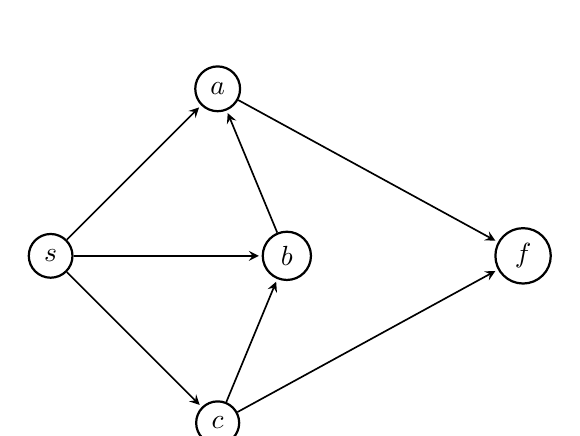
\begin{tikzpicture}[
            > = stealth, % arrow head style
            shorten > = 1pt, % don't touch arrow head to node
            auto,
            node distance = 3cm, % distance between nodes
            semithick % line style
        ]

        \tikzstyle{every state}=[
            draw = black,
            thick,
            fill = white,
            minimum size = 4mm
        ]

        \node[state] (s) {$s$};
        \node[state] (a) [above right of=s] {$a$};
        \node[state] (b) [right of=s] {$b$};
        \node[state] (c) [below right of=s] {$c$};
        \node[state] (f) [right of=b] {$f$};

        \path[->] (s) edge node {} (a);
        \path[->] (s) edge node {} (b);
        \path[->] (s) edge node {} (c);
        \path[->] (b) edge node {} (a);
        \path[->] (c) edge node {} (b);
        \path[->] (c) edge node {} (f);
        \path[->] (a) edge node {} (f);

%        \draw[red, dashed] (1, 2) -- (1, -2);

    \end{tikzpicture}
\caption{A directed graph.}
\end{figure}

\item The directed graph in Figure~\ref{dirgraph} can be represented as the \Verb+LISP+ list:

\begin{lispcode}
((S A) (S B) (S C) (A F) (C B) (B A))
\end{lispcode}

\item We can economize on representation by representing each node as a single list consisting of itself -- as the car of the list -- and collecting all the nodes that are directed from it in the cdr of the list. For instance,

\begin{lispcode}
((S A B C) (A F) (C B) (B A))
\end{lispcode}

\end{uenum}

\subsection{Searching for paths in a graph}

\begin{uenum}
\item We write a program to find paths given a starting point and destination. 

\begin{lispcode}
(defun extend-path (path &optional (graph *graph1*))
  (let ((neighbors (cdr (assoc (car path) graph))))
	(mapcar #'(lambda (node)
				(cons node path))
			(remove-if #'(lambda (node) (member node path)) 
					   neighbors))))

(defun search-path (start end graph
						  &key
						  (mode 'bf)
						  (agenda (list (list start))) 
						  result
						  (current (car agenda)))
  (cond ((endp agenda) result)
		((equal end (car current))
		 (search-path start end graph 
					  :agenda (cdr agenda)
					  :result (cons (reverse current) result)
					  :mode mode))
		(t
		  (search-path start end graph 
					  :agenda (if (equal mode 'df) 
								(append 
								 (extend-path current graph) 
								 (cdr agenda))
								(append 
								 (cdr agenda)
								 (extend-path current graph)))
					  :result result
					  :mode mode))))
\end{lispcode}


\end{uenum}


\item A list headed by \Verb+FORMAT+ is evaluated specially. The first argument to \Verb+FORMAT+ -- \Verb+T+ in the present case -- is there to tell \Verb+FORMAT+ to print the third argument -- \Verb+"Hello"+, a string -- to the screen. (Note that \Verb+LISP+ does not turn this to uppercase, because it is not a symbol, it is a string.) The \Verb+NIL+ you see coming after this is the value the \Verb+FORMAT+ expression returns. Every \Verb+LISP+ expression returns a value. \Verb+FORMAT+ not only returns a value, but also does something -- it has a \cttr{side effect}. We will talk more on this. 

\item With \Verb+FORMAT+ you can do more interesting things. One is to insert values to your string; try and examine the following to understand what is going on.

\begin{lispcode}
(format t "Hello ~A" 'world)
(format t "Hello ~A" (cadr '(world universe)))
(format t "Hello ~A, I'm here!" (cadr '(world universe)))
(format t "Does ~A love ~A?~% or is it the other way around?"
		'john 'mary)
(format t "~A times ~A is ~A" 2 3 (* 2 3))
\end{lispcode}

\item There are many ways to manipulate \Verb+FORMAT+ expressions, but most important ones are \Verb+~A+ to insert values and \Verb+~%+ to have line breaks.


\item Let us now write a function that checks for membership in a list. \Verb+LISP+ already has the function \Verb+MEMBER+ for this purpose, but writing your own versions of such built-in functions is an invaluable educational practice. Here we encounter a new thing, the \Verb+RETURN+ expression: 

\begin{lispcode}
(defun member2 (elm lst)
  (dolist (i lst)
	(if (equal i elm)
	  (return t))))
\end{lispcode}

We basically check each element in \Verb+LST+ as to whether it is \Verb+EQUAL+ to \Verb+ELM+, and if we discover that the equality holds we terminate the iteration by a \Verb+RETURN+ expression. \Verb+RETURN+ is also a special function: it terminates the block that is in and makes the block evaluate to its first argument, which is \Verb+T+ in the present case.


%\begin{comment}%start

% \section{Cognition, computation, computers, programs}
% 
% \subsection{Cognition and computation}
% 
% \begin{uenum}
% 
% \item Cognitive Science: mind/brain is analogous to software/hardware. 
% 	\begin{uenumi}
% 	\item Various names: ``the computational view of mind,'' ``information processing psychology,'' ``the computational theory of mind,'' or simply ``computationalism.''
% 	\item The analogy is usually far from strict and there are many varieties.
% 	\item For instance: ``mind/cognition is computation'' versus ``mind/cognition is computable.''
% 	\end{uenumi}
% 
% \item Why we need computationalism?
% 
% 	\begin{uenumi}
% 	\item Compare the tasks:\footnote{We gloss over a potential objection to the legitimacy of this comparison, given the huge difference between the well-definedness of the questions.}
% 
% 		\begin{itemize}
% 		\item Predicting the trajectory of celestial bodies, say the motion of the earth in the next six hours.
% 		\item Predicting the next move of a chess player at a given state of the game.
% 		\end{itemize}
% 
% 	\item \ctnm[103]{crane03}: ``The planets do not `compute' their orbits from the input they receive: they just move.''
% 	\item In the case of chess, physical description and physical laws are helpless.  The source of helplessness is twofold: (i) The state of a chess game has infinitely many physical realizations, and whether a physical state is a game state is dependent on  whether or not some cognitive agents interpret the ``scene'' as a chess game or not. Therefore a function from physical description to game state is at best extremely complex. (ii) Even if we find a way from physical description to game state, the physical description of rule-based behavior would be a function of the particular realization function (the mapping from physics-to-chess states) at that particular occasion \cttxp{pylyshyn84}.
% 
% 	\end{uenumi}
% 
% \item Computation and cognition share an essential property: both operate on rules and
% representations, yet are based on (instantiated by)  physical causal systems.
% What is happening in a computer and mind/brain are quite similar.
% 
% \hitem{Levels} (more on this below):
% 
% \begin{itemize}
% \item[i.] physical (device)
% \item[i.] symbolic (syntactic) 
% \item[iii.] intentional (semantic)
% \end{itemize}
% 
% \end{uenum}
% 
% \secsep
% 
% \subsection{What is (symbolic) computation?}
% 
% \begin{uenum}
% \item Symbols (or signs) and signification are central concepts in language, logic, and computation.
% 	\begin{uenumi}
% 	\item Take signification as a three-part relation:
% 
% 	\begin{tikzpicture}[node distance=60pt]
% 
% 	\node (usr) {user};
% 	\node [below left of=usr] (sym) {symbol};
% 	\node [below right of=usr] (ob) {object};
% 
% 	\draw [<->] (sym) -- (ob);
% 	\draw [<->] (usr) -- (sym);
% 	\draw [<->] (usr) -- (ob);
% 
% 	\end{tikzpicture}
% 
% 	\begin{itemize}
% 	\item A user uses a sign to \uterm{refer} to an object.
%  	\item A sign \uterm{denotes} an object.
% 	\item A user has certain \uterm{intentions} about an object. 
% 	\end{itemize}
% 
% 
% 	\item A sequence of binary digits (bits) is a symbolic representation: $$001011010100111000000010$$
% 
% 	\end{uenumi}
% 
% \item A computational process is a sequence of manipulations performed over
% symbolic representations.
% 	\begin{uenumi}
% 	\item Example: the process by which you flip the digits of the
% representation above, one at a time is a computational process.
% 	\end{uenumi}
% 
% \end{uenum}
% 
% \secsep
% 
% \subsection{Abstract machines (optional)}
% 
% \begin{figure}
% \begin{center}
% \begin{tikzpicture}[scale=0.7]
% \tikzstyle{every path}=[very thick]
% 
% \edef\sizetape{0.7cm}
% \tikzstyle{tmtape}=[draw,minimum size=\sizetape]
% \tikzstyle{tmhead}=[arrow box,draw,minimum size=.5cm,arrow box
% arrows={east:.25cm, west:0.25cm}]
% 
% %% Draw TM tape
% \begin{scope}[start chain=1 going right,node distance=-0.15mm]
%     \node [on chain=1,tmtape,draw=none] {$\ldots$};
%     \node [on chain=1,tmtape] {\#};
%     \node [on chain=1,tmtape] (input) {\#};
%     \node [on chain=1,tmtape] {0};
%     \node [on chain=1,tmtape] {1};
%     \node [on chain=1,tmtape] {1};
%     \node [on chain=1,tmtape] {0};
%     \node [on chain=1,tmtape] {1};
%     \node [on chain=1,tmtape] {\#};
%     \node [on chain=1,tmtape,draw=none] {$\ldots$};
%     \node [on chain=1] {\textbf{Input/Output Tape}};
% \end{scope}
% 
% %% Draw TM Finite Control
% \begin{scope}
% [shift={(3cm,-5cm)},start chain=circle placed {at=(-\tikzchaincount*60:1.5)}]
% \foreach \i in {q_0,q_1,q_2,q_3,\ddots,q_n}
% 	\node [on chain] {$\i$};
% 
% % Arrow to current state
% \node (center) {};
% \draw[->] (center) -- (circle-2);
% 
% \node[rounded corners,draw=black,thick,fit=(circle-1) (circle-2) (circle-3) 
%       (circle-4) (circle-5) (circle-6),
% 			label=below:\textbf{Finite Control}] (fsbox)
% 		{};
% \end{scope}
% 
% %% Draw TM head below (input) tape cell
% \node [tmhead,yshift=-.3cm] at (input.south) (head) {$q_1$};
% 
% %% Link Finite Control with Head
% \path[->,draw] (fsbox.north) .. controls (4.5,-1) and (0,-2) .. node[right] 
% 			(headlinetext)
%  			{} 
% 			(head.south);
% \node[xshift=3cm] at (headlinetext)  
% 			{\begin{tabular}{c} 
% 				\textbf{Read/Write Head} \\  
% 				\textbf{(moves in both directions)} 
% 			 \end{tabular}};
% 
% \end{tikzpicture}
% \end{center}
% \caption{A Turing Machine}
% \end{figure}
% 
% 
% \begin{itemize}
% \item A Turing Machine (TM) is specified as a quintuple $\langle \Sigma,Q, q_0,q_H, \omega
% \rangle$, where 
% \begin{center}
% \begin{tabular}{lp{200pt}}
% $\Sigma$ & is an alphabet of admissible symbols (including a symbol for
% blank cells);\\
% $Q$ & is a finite set of internal states;\\
% $q_0\in Q$ & is the starting state;\\ 
% $q_H\in Q$ & is the halting state;\\
% $\omega$ & is the state transition function of the form:
% $$
% \langle q,\sigma \rangle \mapsto \langle q',\sigma',M \rangle
% $$
% where $q$ and $q'$ are states, $\sigma$ and $\sigma'$ are symbols, and $M \in \{-1,0,1\}$, for `move left', `don't move', and  `move right', respectively. 
% \end{tabular}
% \end{center}
% \end{itemize}
% 
% \begin{uexample}
% A TM that decides whether its input is a palindrome. Let $\#$ be the blank symbol, $q_0$ the initial, and $q_8$ the halting state.
% 
% $$
% \begin{array}{lcl}
% \langle q_0,\# \rangle & \mapsto & \langle q_8,1,0 \rangle \\
% \langle q_0,0 \rangle & \mapsto & \langle q_1,\#,1 \rangle \\
% \langle q_0,1 \rangle & \mapsto & \langle q_2,\#,1 \rangle \\
% \langle q_1,\#\rangle & \mapsto & \langle q_3,\#,-1 \rangle \\
% \langle q_1,0 \rangle & \mapsto & \langle q_1,0,1 \rangle \\
% \langle q_1,1 \rangle & \mapsto & \langle q_1,1,1 \rangle \\
% \langle q_2,\#\rangle & \mapsto & \langle q_4,\#,-1 \rangle \\
% \langle q_2,0 \rangle & \mapsto & \langle q_2,0,1 \rangle \\
% \langle q_2,1 \rangle & \mapsto & \langle q_2,1,1 \rangle \\
% \langle q_3,\#\rangle & \mapsto & \langle q_8,1,0 \rangle \\
% \langle q_3,0\rangle & \mapsto & \langle q_5,\#,-1 \rangle \\
% \langle q_3,1\rangle & \mapsto & \langle q_7,\#,-1 \rangle \\
% \end{array}
% \quad\quad
% \begin{array}{lcl}
% \langle q_4,\#\rangle & \mapsto & \langle q_8,1,0 \rangle \\
% \langle q_4,0\rangle & \mapsto & \langle q_7,\#,-1 \rangle \\
% \langle q_4,1\rangle & \mapsto & \langle q_5,\#,-1 \rangle \\
% \langle q_5,\#\rangle & \mapsto & \langle q_0,\#,1 \rangle \\
% \langle q_5,0\rangle & \mapsto & \langle q_5,0,-1 \rangle \\
% \langle q_5,1\rangle & \mapsto & \langle q_5,1,-1 \rangle \\
% \langle q_6,\#\rangle & \mapsto & \langle q_0,\#,1 \rangle \\
% \langle q_6,0\rangle & \mapsto & \langle q_6,0,-1 \rangle \\
% \langle q_6,1\rangle & \mapsto & \langle q_6,1,-1 \rangle \\
% \langle q_7,\#\rangle & \mapsto & \langle q_8,0,0 \rangle \\
% \langle q_7,0\rangle & \mapsto & \langle q_7,\#,-1 \rangle \\
% \langle q_7,1\rangle & \mapsto & \langle q_7,\#,-1 \rangle \\
% \end{array}
% $$
% 
% \qed
% \end{uexample}
% 
% 
% \secsep
% 
% \subsection{Hardware/software}
% 
% \begin{figure}
% \begin{center}
% \begin{tikzpicture}[ node distance=2cm,>=latex']
% \tikzstyle{block} = [draw, fill=blue!20, rectangle, 
%     minimum height=3em, minimum width=6em]
% \tikzstyle{control} = [draw, fill=blue!20, rectangle, minimum width=4cm, text centered, node distance=3cm]
% \tikzstyle{register} = [draw, fill=blue!20, rectangle, text centered,text width=2.7cm, minimum width=2.7cm, minimum height=1cm,node distance=2.3cm]
% \tikzstyle{alu} = [draw, fill=blue!20, rectangle, text centered,text width=2.7cm, minimum width=2.7cm, minimum height=1cm,node distance=2.3cm]
% \tikzstyle{memory} = [draw, rectangle, text centered, minimum width=1.5cm, minimum height=4.3cm,node distance=4.3cm]
% \tikzstyle{input} = [draw, rectangle, text centered,text width=2.7cm, minimum width=2.7cm, minimum height=1cm,node distance=2.3cm]
% \tikzstyle{output} = [draw, rectangle, text centered,text width=2.7cm, minimum width=2.7cm, minimum height=1cm,node distance=2.3cm]
% 
%     % We start by placing the blocks
% 	\node [control] (control) {\small Control Unit};
%     \node [register, below left of=control] (reg) {\footnotesize Registers};
%     \node [alu, below right of=control] (alu) {\footnotesize Arithmetic Logic Unit \\ ALU};
%     \node [memory, right of=control] (mem) {\footnotesize Memory};
%     \node [input, above left of=control] (in) {\footnotesize Input Device};
%     \node [output, above right of=control] (out) {\footnotesize Output Device};
% 
%     \draw [<->] (control) --node {} (reg);
%     \draw [<->] (control) --node {} (alu);
%     \draw [<-] (control) --node {} (in);
%     \draw [->] (control) --node {} (out);
%     \draw [<->] (control) --node {} (mem);
% 
% \end{tikzpicture}
% \end{center}
% \caption{Von Neumann architecture}
% \end{figure}
% 
% \begin{uenum}
% 
% \item Most computers we have around are based on  von Neumann\footnote{Named after the mathematician and physicist 
% John von Neumann.} architecture.
% 
% \item VNA consists of \uterm{memory}, \uterm{central processing unit}, and I/O devices.
% 
% \item Memory consists of a sequence of \uterm{cells} (also called \uterm{words}). 
% 	\begin{uenumi}
% 	\item Each cell is of a fixed capacity. 
% 		\begin{uenumii}
% 		\item What we mean by capacity is how many binary digits (bits) a cell can hold. 
% 		\item Bits are thought of in groups of 8's; 8 bits $=$ 1 \uterm{byte}. 
% 		\item A single byte can hold $2^8$ different values, or symbols, if you like.  
% 		\end{uenumii}
% 	\item Each cell of memory has a unique \uterm{address}, itself a binary number.  
% 	\end{uenumi}
% \item The two basic components, CPU and memory, communicate through three
% channels:
% 	\begin{itemize}
% 	\item[i.] A collection of wires called \uterm{address bus};
% 	\item[ii.] Another collection of wires called \uterm{data bus};
% 	\item[iii.] A single wire called \uterm{R/W line}, the status of which
% 	signals whether CPU wants to write to or read from the memory.
% 	\end{itemize}
% 
% \item The address bus and the R/W line are one way channels. The value is always
% dictated by the CPU. The data bus is a two-way channel.
% 
% \item The two basic interactions between CPU and Memory go as follows:
% 	\begin{itemize}
% 	\item CPU sets the address bus and R/W line	to W. In
% 	that case it also sets the data bus. Obviously, this amounts to dictating to
% 	write the data to the given address in memory.
% 	\item CPU sets the address bus and R/W line to R. In this case it is the
% 	memory that sets the data bus in accord with the data located at the address
% 	provided by CPU; this is reading from memory.
% 	\end{itemize}
% 
% \item CPU itself also has some local memory slots. These are called
% \uterm{registers}. Access to registers is faster than access to memory. But
% there is a reason to keep the size of the CPU small, therefore there are a
% limited number of registers, which are used to store intermediate results of
% computations and some frequently used information. 
% 
% \item The computation unit of CPU is \uterm{arithmetic logic unit} (ALU, for
% short.) ALU is responsible for arithmetic and logical operations.
% 
% \item CPU feeds on \uterm{instructions}. Some typical types of instructions are:
% 
% \begin{enumerate}[label=\roman*.]
% \item Store the number at the register $X$ at the memory address $Y$;
% \item Fetch the number at the address $X$  and store it at the register $Y$;
% \item Add the number at address $X$ to the number at address $Y$, and store the
% result at address $Z$;
% \item Compute the bitwise \emph{and} of the numbers at addresses $X$  and $Y$,
% and store the result at the address $Z$;
% \item If the contents of the register $X$ and $Y$ are not identical, go to
% address $Z$;
% \item Jump to the address $X$;
% \item and so on.
% \end{enumerate}
% 
% \item
% \uterm{Stored-program} concept
% 	\begin{enumerate}[label=\alph*.]
% 	\item Not only data but also instructions are represented as numbers;
% 	\item Programs are stored in memory; they can be read and written just like data. 
% 	\end{enumerate}
% 
% % \item This doesn't have to be this way; you can have a rigidly programmed
% % hardware. 
% % 
% % \item What, if any, could be the significance of this distinction for the brain and
% % cognition?
% 
% 
% \item A central aspect of a computational system is \uterm{flow of control}.
% Some instructions have \emph{go to} or \emph{jump}, which sends the control to
% another instruction. But other instructions lack such a mechanism for flow of
% control. 
% 
% \item There is a special register called \uterm{program counter}, where the
% address of the next instruction is kept.
% 
% \item CPU operates through a sequence of
% cycles. Each cycle begins by fetching a binary description of what to do, an
% \uterm{instruction} from an address in Memory. Following this, CPU understands,
% or technically speaking, \uterm{decodes} the instruction. The next step is to
% \uterm{execute} the instruction. This completes a single cycle, which is
% followed by reading the next instruction from Memory.\footnote{Cycles are called
% `fetch-decode-execute' or `instruction cycle'.}
% 
% \end{uenum}
% 
% \secsep
% 
% \subsection{Levels of programming}
% 
% \begin{uenum}
% 
% \item Computers operate on numbers, in the sense that the functional
% architecture of the machines get their instructions as binary numbers organized
% into expressions of \uterm{machine code}.
% 
% \item Given a functional architecture, say VNA, a straightforward specification
% would be to code the memory byte-by-byte (writing \uterm{machine code}); so that
% CPU ``knows'' what to do in each possible state of the process.   
% 
% \item Example of an addition instruction:
% 
% \begin{Verbatim}
% 000000 10001 10010 01000 00000 1000000
% \end{Verbatim}
% 
% \item A machine code instruction is organized into \uterm{fields} with different
% meanings.
% 
% \item Some levels up the machine code is the \uterm{assembly} language. The above
% machine code takes the form:
% 
% \begin{Verbatim}
% 
% add $s1,$t1,$t
% 
% \end{Verbatim}
% \begin{comment} This is needed to fix syntax highlighting problem due to unmatched $ \end{comment}
% 
% 
% 
% \item Assembly level lies between high-level languages and machine code.
% 
% \item[] A simple while loop in C:
% 
% \begin{ucodeframe}
% \begin{Verbatim}
% while (save[i] == k) {
% 	i = i + 1;
% 	}
% \end{Verbatim}
% \end{ucodeframe}
% 
% \item[] Assuing that \Verb+i+ and \Verb+k+ are stored in registers \Verb+$s3+
% and \Verb+$s5+, and the array \Verb+save+ starts at the memory address stored in
% \Verb+$s6+, the above C code is \uterm{compiled} to the following assembly
% code (for MIPS):
% 
% 
% \begin{ucodeframe}
% \begin{Verbatim}
% Loop:  sll $t1,$s3,2
%        add $t1,$t1,$s6
%        lw  $t0,0($t1)
%        bne $t0,$s5,Exit
%        add $s3,$s3,1
%        j   Loop
% Exit:
% \end{Verbatim}
% \end{ucodeframe}
% 
% \item A computational process can be specified at various levels.
% 
% \end{uenum}
% 
% 
% \secsep
% \subsection{More into hardware}
% 
% \begin{uenum}
% 
% \item The basic building block of modern computer is the transistor.\footnote{The figures in this subsection are taken from \cttx{tanenbaum99}.} Transistors are organized into logic gates.
% 
% \begin{center}
% \includegraphics[scale=0.7]{img/transistor.png}
% \end{center}
% 
% 
% \begin{center}
% \includegraphics[scale=0.7]{img/gates.png}
% \end{center}
% 
% 
% \begin{center}
% \includegraphics[scale=0.7]{img/xor.png}
% \end{center}
% 
% 
% \item Mechanical addition with circuits:
% 
% \includegraphics[scale=0.7]{img/halfadder.png}
% 
% \includegraphics[scale=0.7]{img/fulladder.png}
% 
% \end{uenum}
% 
% \secsep
% 
% \subsection{Further reading}
% 
% \ctnm{pohlshaw81} is an introduction to computer science, for non-computer scientists.
% \ctnm{tanenbaum99} (or a newer edition) is an accessible book on computer architecture. It also provides a short and nice history of computers.  
% \ctnm{pylyshyn84} is a classic on cognition and computation, from the representational camp. Consult \ctnm{churchlandsejnowski92} for a connectionist approach to the same topic. The last two books are NOT introductory level. For a general introduction, see \ctnm{crane03}.
% 
% 
